%------------------------------------------------------------------------------------------------------------------------
\chapter{試験結果データ管理システムの開発}
\label{sec:chap7}
%------------------------------------------------------------------------------------------------------------------------

本研究では、これまで読み出し試験用に開発されていたシステムの他に、ピクセルモジュールの品質管理の流れの全てをサポートできるように機能の作成を行った。本研究において開発した項目を以下に示す。
\begin{itemize}
  \item[1.] 品質試験結果の表示機能(\ref{sec:hyouji}節)
  \begin{itemize}
    \item 非読み出し試験結果の閲覧機能
    \item ピクセルモジュール特性の閲覧機能
    \item 読み出し試験結果比較機能
  \end{itemize}
  \item[2.] 品質試験結果の管理機能(\ref{sec:kanri}節)
  \begin{itemize}
    \item ピクセルモジュール特性の選択機能
  \end{itemize}
  \item[3.] 中央データベースとローカルデータベースの同期機能(\ref{sec:douki}節)
  \begin{itemize}
    \item ピクセルモジュール情報の登録機能
    \item 品質試験結果のアップロード機能
    \item 品質試験結果のダウンロード機能
  \end{itemize}
\end{itemize}

%------------------------------------------------------------------------------------------------------------------------
\section{品質試験結果の表示機能}
\label{sec:hyouji}
%------------------------------------------------------------------------------------------------------------------------

前章で示したように、多様な利用者がデータベース内のデータを閲覧、操作を実現できることを目標としてウェブアプリケーションの開発を行っている。これまでは読み出し試験に特化した開発が行われていたが、その他の品質試験結果を表示する機能は未実装であった。本研究では、品質試験結果登録用GUIの開発者と協力し、ローカルデータベース内でのデータの保管方法と結果の閲覧機能の開発を行った。さらに、先行研究で開発された読み出し試験結果の解析機能を拡張し、別の試験結果と比較する機能の開発を行った。

本節では、それぞれの機能の概要と各品質試験項目についての結果の閲覧機能について説明する。


%------------------------------------------------------------------------------------------------------------------------
\subsection{非読み出し試験結果閲覧機能の概要}
\label{sec:non-elec-data}
%------------------------------------------------------------------------------------------------------------------------

これまでは読み出し試験結果についての開発を中心に行われており、その他の品質試験結果を表示する機能は未実装であった。ピクセルモジュール次世代器量産におけるの品質試験を管理するためには、非読み出し試験結果を管理する機能が必要である。本研究では、非読み出し試験結果登録用GUIであるQC-helperの開発者と協力し、ローカルデータベース内でのデータの管理方法と結果の閲覧機能の開発を行った。以下に詳細を示す。

\tref{tab:local-collection}に示したように、品質試験結果はMongoDBのQC.resultsというコレクションに保存される。非読み出し試験結果の例を以下に示す。

\begin{lstlisting}[caption=品質試験結果を表すドキュメントの例。以下は質量測定結果の一つを表している。,label=code:nonele, language=C++]
{
  "_id" : ObjectId("6131a0532e16df12955d9c6d"),
  "component" : "60b9dc51d978dc000b9232fc",
  "user" : "kinoshita",
  "address" : "Tokyo Institute of Technology",
  "currentStage" : "MODULETOPCB",
  "testType" : "MASS",
  "sys" : {
    "cts" : ISODate("2021-09-03T04:10:57.338Z"),
    "mts" : ISODate("2021-09-03T04:10:57.338Z"),
    "rev" : 0
  },
  "results" : {
    "property" : {
      "Scale_accuracy" : 0.5,
      "Scale_accuracy_unit" : "g"
    },
    "mass_value" : 1,
    "mass_unit" : "g",
    "comment" : "hoge"
  },
  "dbVersion" : 1.01
}
\end{lstlisting}

先述したように非読み出し試験の結果はQC-helperによってMongoDBに登録される。全ての品質試験結果では上記のドキュメントの\textbf{results}を除く値を共通要素として持ち、品質試験項目によりresultsに格納するパラメータが異なる。

画像やJSON file等のファイルデータの保存はGridFS\cite{mongo}と呼ばれるインターフェースが使用される。GridFSはサイズの大きいファイルの実体を$255\ \si{kB}$サイズのドキュメントに分割して保存する使用である。GridFSは、\textbf{fs.files}と\textbf{fs.chunks}というコレクションを用いてファイルデータを管理する。fs.chunksにファイルを分割して書き込み、fs.filesにファイルのメタデータ(ファイル名、サイズ、fs.chunksにおける分割数等)が書き込まれる。非読み出し試験については、外観検査における高画素画像およびワイヤー配線のためのデータファイルをGridFSによって保存し、QC.resultのドキュメントにfs.filesドキュメントファイルのオブジェクトIDを記録することによって、品質試験結果とデータの関連付けを行っている。


%------------------------------------------------------------------------------------------------------------------------
\subsection{非読み出し試験結果閲覧機能}
\label{sec:non-elec-view}
%------------------------------------------------------------------------------------------------------------------------

非読み出し試験結果のウェブブラウザ出力を\fref{fig:noneleresult}に示す。試験結果をウェブブラウザから閲覧できるように、各ピクセルモジュールのページ(\fref{fig:noneleresult}の左)の下部に登録した品質試験結果の一覧を表示する。この一覧は、初めは試験日時について昇順に表示しているが、
必要に応じて別の項目におけるソートを可能にするため、JavaScriptを利用し動的に処理できるようにした。項目名をクリックするとソートすることが可能であり、クリックする毎に昇順、降順、ソート解除となる。

ブラウザから受け取った信号をもとにデータベース内データの抽出処理を行い、試験結果を適切な形に整形しブラウザに表示する。\cref{code:nonele}に示すように、試験日時や試験場所等の試験結果の基本要素を全ての試験項目について共通要素としてもち、"results"の値のみ試験項目で個別の形式を持つ。そこで、共通項目としては前試験項目について共通の票を出力、品質試験結果については適切な形に整形しブラウザに表示するようにした。\fref{fig:noneleresult}の右図は外観検査についてのウェブブラウザ表示であり、外観検査において問題があると判定された部分の拡大写真のGridFSから抽出し、コメントと共に表示している。その他の品質試験結果の表示画面については付録\ref{sec:A1}にまとめる。

\begin{figure}[tbp]
  \begin{minipage}[b]{0.45\linewidth}
    \centering
    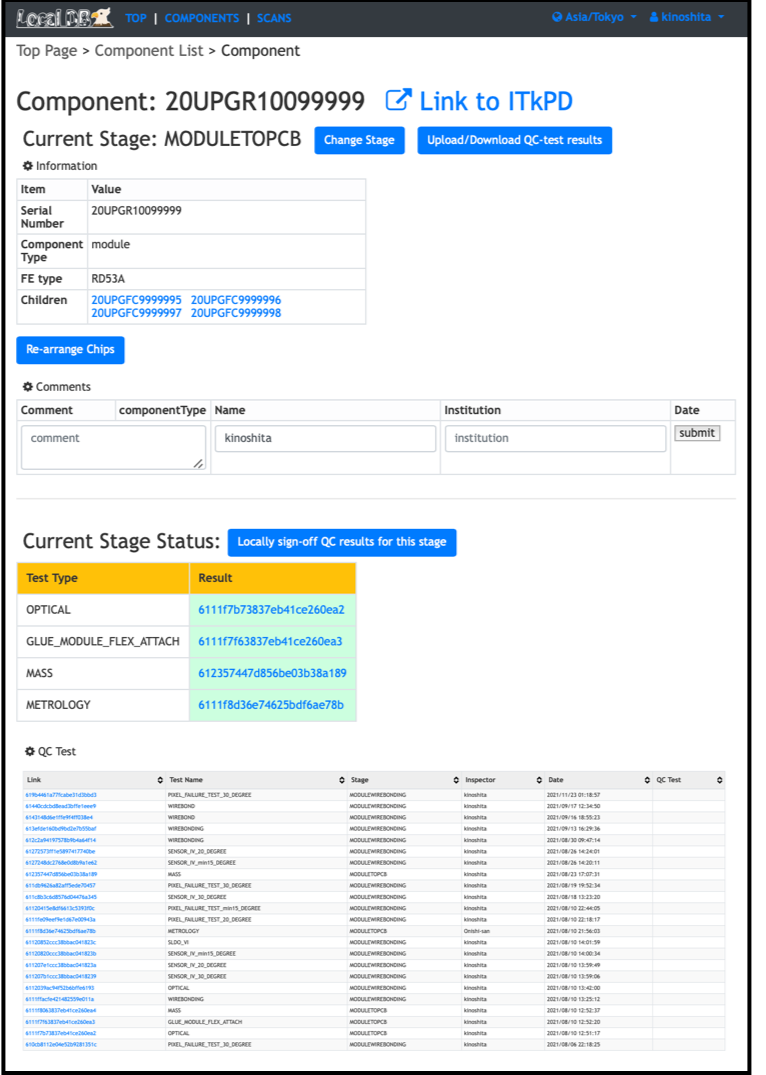
\includegraphics[keepaspectratio, scale=0.5]{componentpage.png}
  \end{minipage}
  \begin{minipage}[b]{0.45\linewidth}
    \centering
    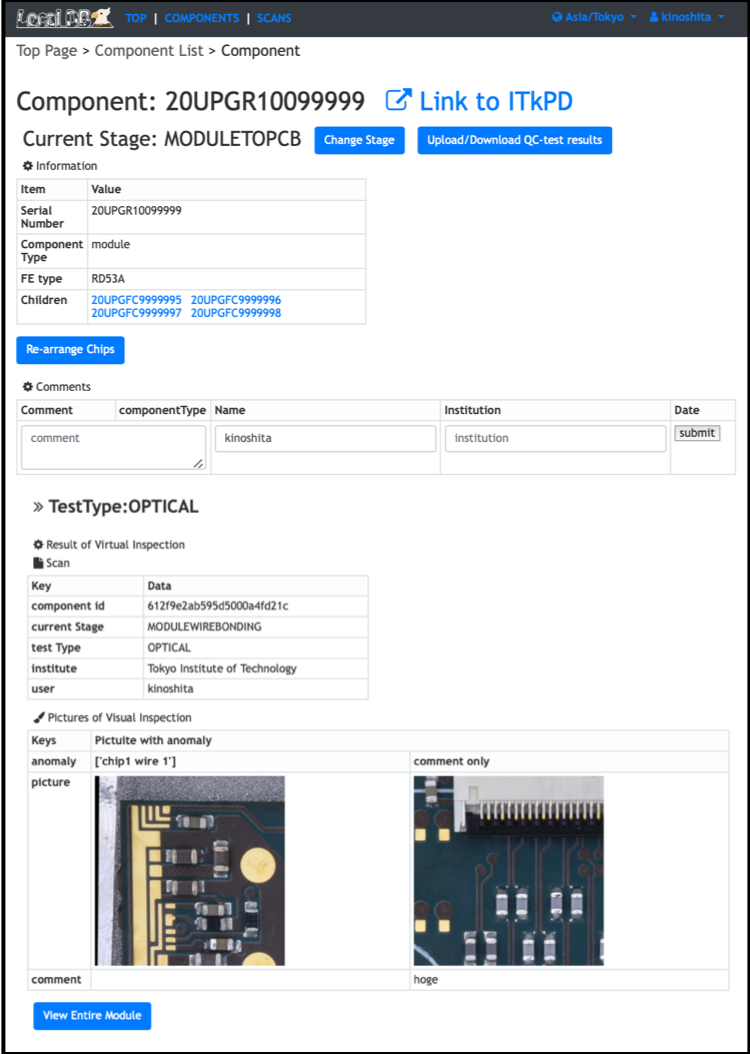
\includegraphics[keepaspectratio, scale=0.5]{viresult.png}
  \end{minipage}
    \caption{非読み出し試験結果のブラウザ出力。}
    \label{fig:noneleresult}
\end{figure}

%------------------------------------------------------------------------------------------------------------------------
\subsection{ピクセルモジュール特性閲覧機能}
\label{sec:prop-view}
%------------------------------------------------------------------------------------------------------------------------

ピクセルモジュールの基本特性について、Iref値やPull-up抵抗値はワイヤー配線後に初めて確認できる。そのため、組み立て工程の途中で情報を更新する必要があり、ローカルデータベースへの基本特性の更新情報は非読み出し試験結果登録用GUIを用いて行われる。\cref{code:moduleprop}に基本特性を管理するドキュメントを示す。基本特性に関する情報はMongoDBの\textbf{QC.module.prop}というコレクションに保存される。内容は品質試験結果を表すコレクションであるQC.resultsと同じであるため、品質試験結果を表すウェブページと同様の処理を行い特性情報を閲覧することができる。基本特性の表示画面については付録\ref{sec:A2}にまとめる。

\begin{lstlisting}[caption=ピクセルモジュールの基本特定更新情報を表すドキュメント。,label=code:moduleprop, language=C++]
{
  "_id" : ObjectId("613ec032f5194763373ddad1"),
  "component" : "6138924058c2e3000a0db59d",
  "user" : "kinoshita",
  "address" : "Tokyo Institute of Technology",
  "currentStage" : "MODULEWIREBONDING",
  "testType" : "IREFTRIM_FE",
  "sys" : {
    "cts" : ISODate("2021-09-13T03:06:25.499Z"),
    "mts" : ISODate("2021-09-13T03:06:25.499Z"),
    "rev" : 0
  },
  "results" : {
    "value" : {
      "chip1" : "1000",
      "chip2" : "1000",
      "chip3" : "1000",
      "chip4" : "1000"
    },
    "comment" : "hoge"
  },
  "dbVersion" : 1.01
}
\end{lstlisting}

%------------------------------------------------------------------------------------------------------------------------
\subsection{読み出し試験結果比較機能}
\label{sec:elec-hikaku}
%------------------------------------------------------------------------------------------------------------------------

%読み出し試験は組み立てたピクセルモジュールの性能を評価する上で重要な品質試験であり、\tref{tab:pixel-failure}の基準に基づきピクセル応答評価を行う。
読み出し試験は組み立てたピクセルモジュールの性能を評価する上で重要な品質試験であり、各ピクセルが正常に動作していることを確認する必要がある。\tref{tab:pixel-failure}に基づきピクセル応答評価機能が先行研究\cite{oku}によって開発された。ピクセル応答評価機能は以下の流れで処理が行われる。
\begin{itemize}
  \item[1. ] データベースから解析するためのデータファイルを取得し、キャッシュディレクトリに保存
  \item[2. ] 作成したファイルを読み込み、ピクセル解析を実行し、結果値やプロットをafter\_analysis.rootと言う名前のファイルにまとめる
  \item[3. ] after\_analysis.rootにまとめられた結果をPNGの画像に変換し出力
\end{itemize}

ピクセル応答評価機能を応用し、二つの結果を比較できる機能の開発を行った。ピクセル解析を行うためにCERNが提供している解析フレームワークであるROOTを使用している。ROOTを用いて作成したafter\_analysis.rootおいてピクセルごとに解析結果がまとめられており、このファイルを利用することにより2つの結果を比較することができる。ピクセル解析結果を\fref{fig:badsum}に示し、各評価基準における不良ピクセルの分布を\fref{fig:badpixel}に示す。

\begin{figure}[tbp]
 \begin{minipage}{0.33\hsize}
  \begin{center}
   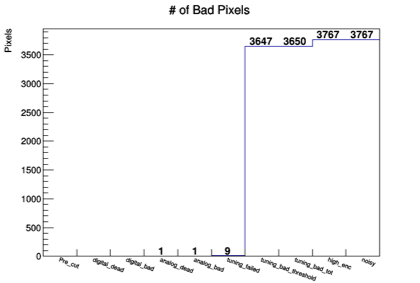
\includegraphics[width=50mm]{sum_after.png}
  \end{center}
 \end{minipage}
 \begin{minipage}{0.33\hsize}
 \begin{center}
  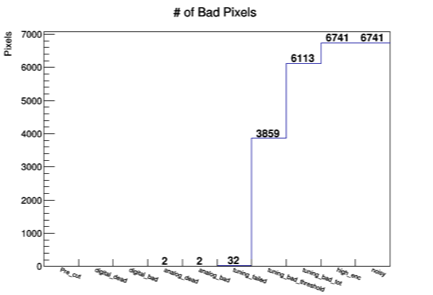
\includegraphics[width=50mm]{sum_before.png}
 \end{center}
 \end{minipage}
 \begin{minipage}{0.33\hsize}
 \begin{center}
  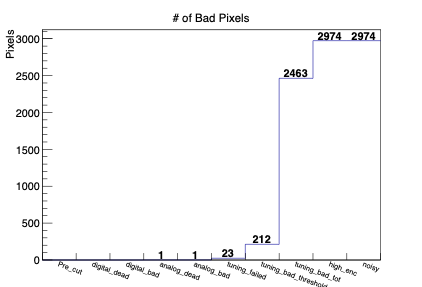
\includegraphics[width=50mm]{sum_diff.png}
 \end{center}
 \end{minipage}
 \caption{ピクセル応答評価機能を用いて作成したピクセル解析結果(左・中央)と2つの差分を用いた比較結果。横軸は評価基準、縦軸は該当する不良ピクセル数を表す。}
 \label{fig:badsum}
\end{figure}

\begin{figure}[tbp]
 \begin{minipage}{0.33\hsize}
  \begin{center}
   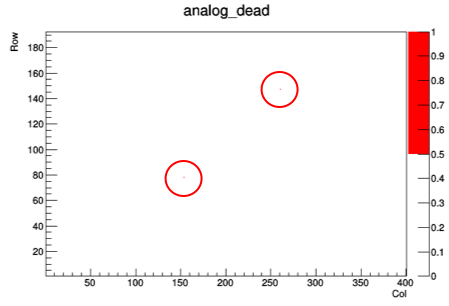
\includegraphics[width=50mm]{bad_before.png}
  \end{center}
 \end{minipage}
 \begin{minipage}{0.33\hsize}
 \begin{center}
  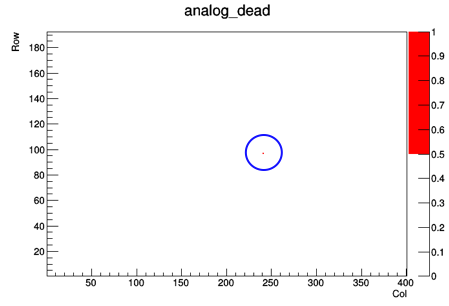
\includegraphics[width=50mm]{bad_after.png}
 \end{center}
 \end{minipage}
 \begin{minipage}{0.33\hsize}
 \begin{center}
  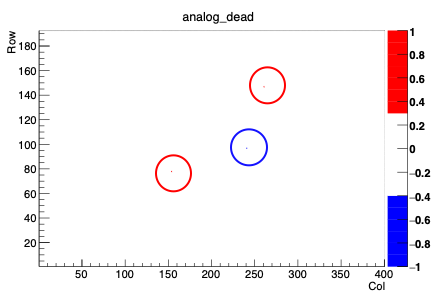
\includegraphics[width=50mm]{bad_diff.png}
 \end{center}
 \end{minipage}
 \caption{ピクセル解析結果における不良ピクセルの分布(左・中央)と2つの差分を用いた比較結果。各図は二次元ヒストグラムであり、横軸はASICにおける各ピクセルの列番号、縦軸は行番号を示している。}
 \label{fig:badpixel}
\end{figure}

この機能を用いることにより、温度サイクル試験におけるモジュールへの熱応力により発生するバンプ部の剥がれが発生した際に、1つ前の組み立て工程でバンプ剥がれが見られるかを確認するということに役に立つ。バンプ剥がれが発生したピクセルモジュールについての読み出し試験結果を\fref{fig:bumphagare}に示す。\fref{fig:bumphagare}はX線を用いて行ったSouceスキャンについての分布である。この図の二次元ヒストグラムの左上の領域にヒット数が無いことから、この部分のバンプが剥がれてしまっていると予想される。このような構造が見つかった際に1つ前の組み立て工程における試験結果と比較し、温度サイクル試験によりバンプ剥がれが生じたかを確認することができる。

しかし、先行研究において開発されたピクセル応答評価機能はSourceスキャンを含むバンプ確認試験に対応していない。そのため、ピクセル応答評価機能を改良し、バンプの接続確認のために必要な解析機能をローカルデータベースに実装する必要がある。


\begin{figure}[tbp]
  \centering
  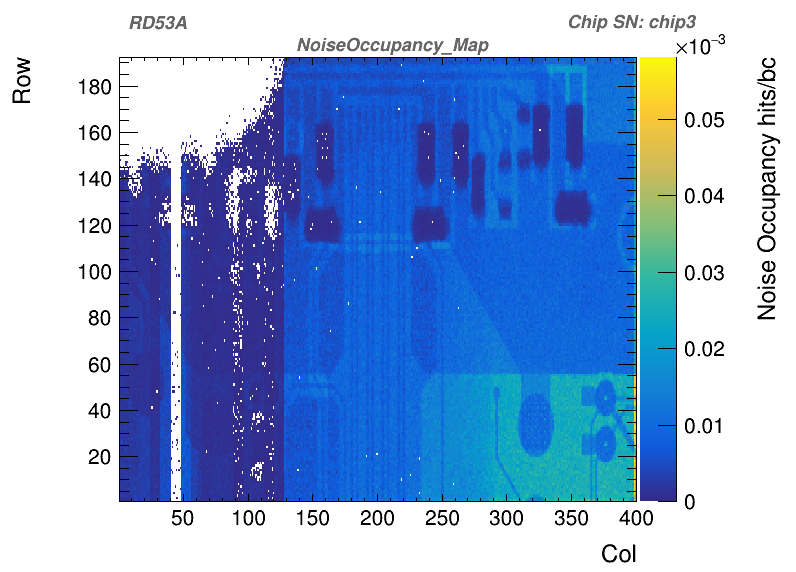
\includegraphics[height=7cm,keepaspectratio]{bumphagare.png}
  \caption[バンプ剥がれが発生したピクセルモジュールについての読み出し試験結果]{バンプ剥がれが発生したピクセルモジュールについての読み出し試験結果。}
  \label{fig:bumphagare}
\end{figure}



%------------------------------------------------------------------------------------------------------------------------
\section{品質試験結果の管理機能}
\label{sec:kanri}
%------------------------------------------------------------------------------------------------------------------------

ローカルデータベースの中でピクセルモジュールの組み立て工程の管理及び各工程に対応する品質試験の選択機能が先行研究\cite{oku}によって開発された。本機能は各ピクセルモジュールが中央データベースで定義された枠組みに準拠して、組み立て工程および品質試験を適切に行うことを目標に開発が進められている。さらに、測定の失敗などでローカルデータベースに保存された不要な品質試験結果を中央データベースに同期しないために、本結果を1つ選択する必要がある。このような機能も先行研究によって開発が進められてきた。

先行研究において開発されたピクセルモジュールの組み立て工程に対して結果を選択する機能の流れを\fref{fig:sign-off}に示す。
\begin{figure}[tbp]
  \centering
  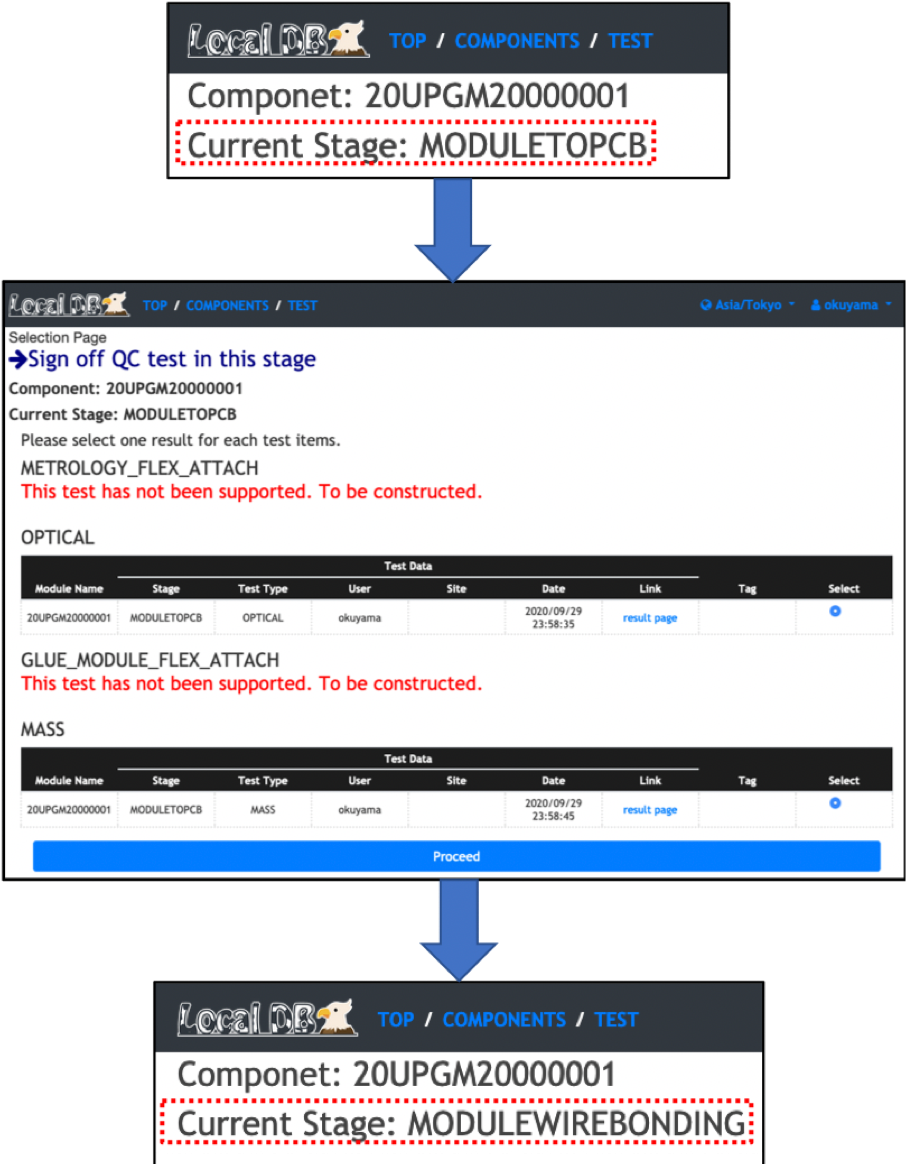
\includegraphics[height=15cm,keepaspectratio]{signoff.png}
  \caption[結果選択画面及び組み立て工程表示の例]{結果選択画面及び組み立て工程表示の例\cite{oku}。図の上部で組み立て工程が “MODULETOPCB” である。図の中部において品質試験結果選択処理を行なっており、この図では “OPTICAL”と “MASS”の結果を選択している。この時、ローカルデータベース内部では選択された結果にタグ付けがなされる。これらの結果は中央データベースと同期される。また結果選択後は組み立て工程が自動的に更新される。図の下部では”MODULEWIREBONDING”になっていることが分かる。}
  \label{fig:sign-off}
\end{figure}

MongoDBの\textbf{QC.module.status}というコレクションを用いて、ピクセルモジュールの組み立て工程の情報が管理される。あるピクセルモジュールの組み立て工程を管理するためのドキュメントの一部を以下に示す。
\begin{lstlisting}[caption=ピクセルモジュールの組み立て工程を管理するためのドキュメントの一部。,label=fuga, language=C++]
{
  "component": "5fa79114e615fa000a1a5976",
  "currentStage" : "MODULEWIREBONDPROTECTION",
  "QC_results" : {
    "MODULETOPCB" : {
      "OPTICAL" : "6111f7b73837eb41ce260ea2",
      "GLUE_MODULE_FLEX_ATTACH" : "6111f7f63837eb41ce260ea3",
      "MASS" : "612357447d856be03b38a189",
      "METROLOGY" : "6111f8d36e74625bdf6ae78b"
    },
    "MODULEWIREBONDING" : {
      "WIREBONDING" : "613efde160bd9bd2e7b55baf",
      "WIREBOND" : "61440cdcbd8ead3bffe1eee9",
      "OPTICAL" : "6112039ac94f52b6bffe6193",
      "SENSOR_IV_30_DEGREE" : "611c8b3c6d8576d04476a345",
      "SENSOR_IV_20_DEGREE" : "61272573ff1e5897417740be",
      "SENSOR_IV_min15_DEGREE" : "6127248dc2768e0d8b9a1e62",
      "SLDO_VI" : "61120852ccc38bbac041823c",
      "PIXEL_FAILURE_TEST_30_DEGREE" : "619b4461a77fcabe31d3bbd3",
      "PIXEL_FAILURE_TEST_20_DEGREE" : "6111fe09eef9e1d67e00943a",
      "PIXEL_FAILURE_TEST_min15_DEGREE" : "61120415e8df6613c5393f0c"
    },
    "MODULEWIREBONDPROTECTION" : {
      "POTTING" : "-1",
      "OPTICAL" : "-1",
      "MASS" : "-1",
      "SENSOR_IV" : "-1",
      "REGISTER_TEST" : "-1",
      "READOUT_IN_BASIC_ELECTRICAL_TEST" : "-1"
    }
  }
}
\end{lstlisting}

QC.module.statusのドキュメントはピクセルモジュールごとに作成される。ドキュメント内の"currentStage"にそのピクセルモジュールの現在の工程についての情報を保持し、\fref{fig:sign-off}で選択した結果は"QC\_results"にそのドキュメントを表すオブジェクトIDを記録することによって、品質試験結果との関連付けを行っている。

この機能は品質試験結果のみに対応しており、ワイヤー配線後に更新を行うピクセルモジュール特性についての管理機能は未実装であった。先行研究で開発された選択機能を改良し、ピクセルモジュール特性を選択する機能の開発を行った。
本研究で開発した機能を以下に示す。

%------------------------------------------------------------------------------------------------------------------------
\subsection{ピクセルモジュール特性の選択機能}
\label{sec:prop-sentaku}
%------------------------------------------------------------------------------------------------------------------------

ワイヤー配線後に決まるピクセルモジュールの基本特性を管理するために、MongoDB内に新たなコレクションを定義した。基本特性の本結果を管理するコレクションとして\textbf{QC.prop.status}を定義し、\cref{code:modulepropstatus}に示すようなドキュメントを作成、保存する。"QC\_properties"にそれぞれの特性項目とその結果を表すオブジェクトIDを記録することにより、特性結果が管理されている\textbf{QC.module.prop}のドキュメントとの関連付けを行う。


\begin{lstlisting}[caption=ピクセルモジュールの組み立て工程を管理するためのドキュメントの一部。,label=code:modulepropstatus, language=C++]
{
  "_id" : ObjectId("611a1c039c1b5786d950a17c"),
  "proddbVersion" : 1.02,
  "component" : "60d426d8b33600000af63e5b",
  "currentStage" : "MODULEWIREBONDING",
  "status" : "created",
  "QC_properties" : {
    "RD53A_PULL-UP_RESISTOR" : "61120d26ccc38bbac0418240",
    "IREFTRIM_FE" : "61120c00ccc38bbac041823e",
    "ORIENTATION" : "61120c0fccc38bbac041823f"
  }
}
\end{lstlisting}

\fref{fig:sign-off}に示した組み立て工程に対して本結果を選択する機能に加え、組み立て工程がワイヤー配線であれば基本特性の測定結果を選択できるようにした。基本特性を選択するウェブブラウザ上の表示を\fref{fig:sign-off-prop}に示す。この機能を用いて選択した基本特性結果のIDが\cref{code:modulepropstatus}の"QC\_properties"の各特性項目の欄に記録される機能となっている。ここで記録された結果が、ワイヤー配線工程における品質試験結果と同時に中央データベースへ同期される。

\begin{figure}[tbp]
  \centering
  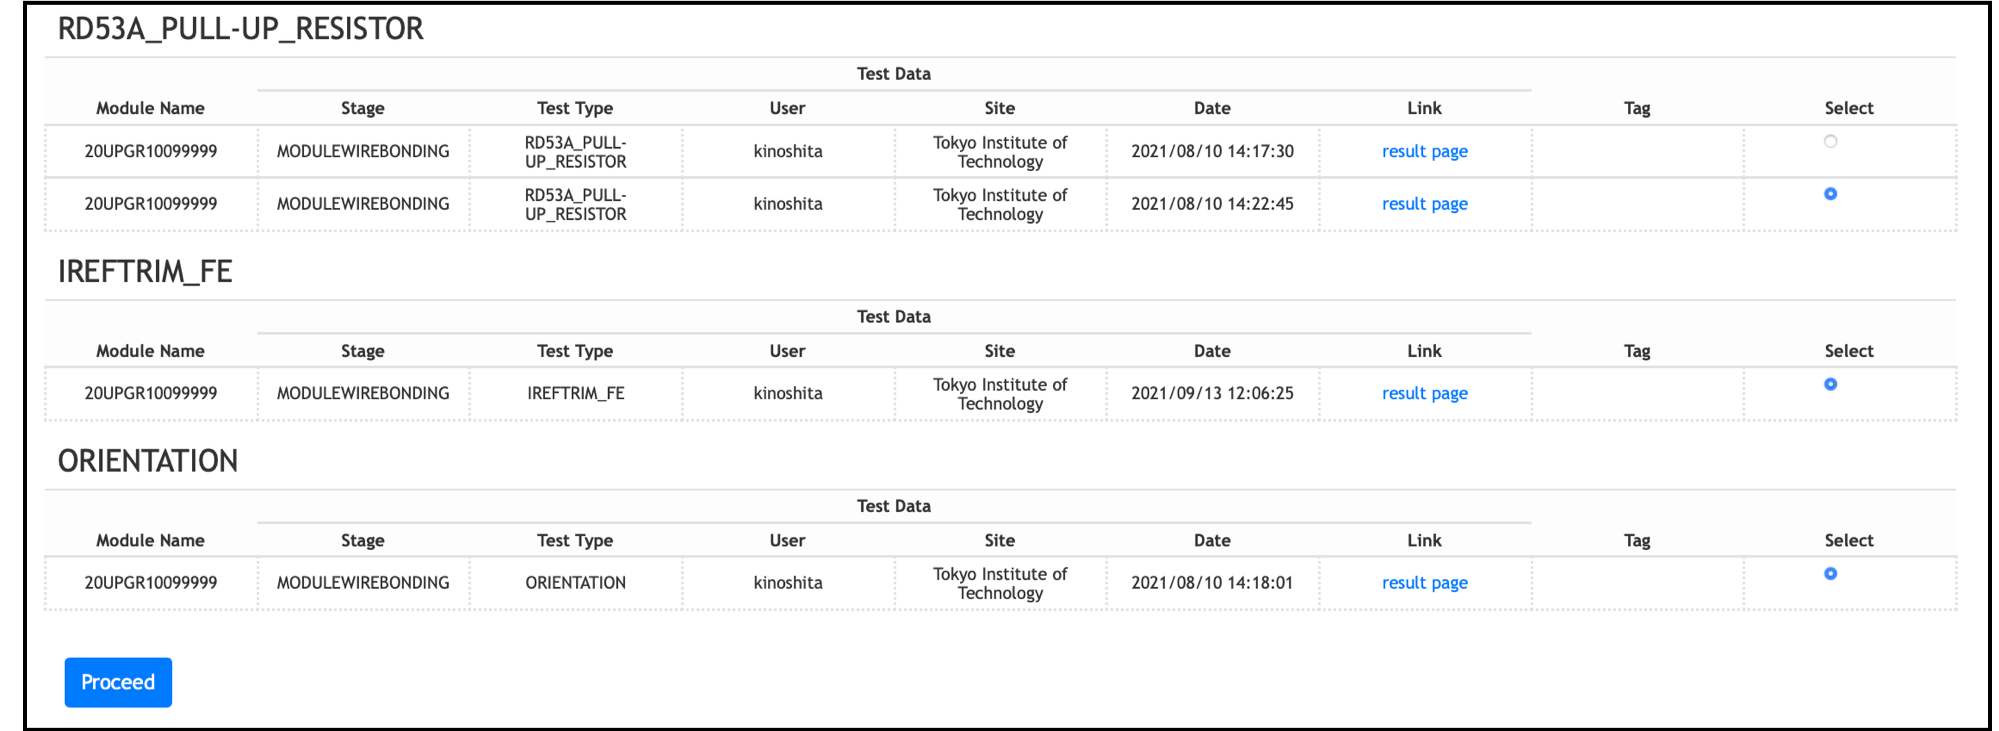
\includegraphics[height=5cm,keepaspectratio]{signoffprop.png}
  \caption[ピクセルモジュールの基本特性選択画面]{ピクセルモジュールの基本特性選択画面。}
  \label{fig:sign-off-prop}
\end{figure}

%------------------------------------------------------------------------------------------------------------------------
\section{中央データベースとローカルデータベースの同期機能}
\label{sec:douki}
%------------------------------------------------------------------------------------------------------------------------

中央データベースにおいてピクセルモジュールの構成部品情報や品質試験結果を管理するために、中央データベースにそれらについての構造を定義する必要がある。中央データベースにおける構造の定義、および実装の大部分は先行研究\cite{oku}によって行われた。さらに、現在行われている試作器を用いた組み立て工程の試験を通して定義された構造の見直しが行われている。構造の再定義のために、ピクセルモジュール開発グループ内で国際的に議論を行いながら、構造の実装を行った。

ピクセルモジュールの情報や品質試験結果を中央データベースに共有するために、中央データベースとローカルデータベース間のデータ共有機能を開発する必要がある。
中央データベースとの通信のために、中央データベースが開発、提供しているPythonパッケージを用いた。

\begin{figure}[tbp]
  \centering
  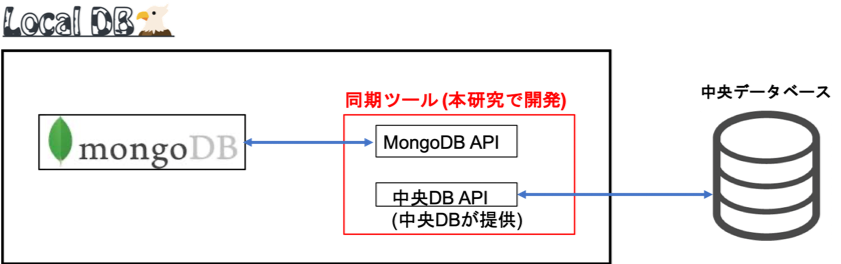
\includegraphics[height=3cm,keepaspectratio]{doukitool.png}
  \caption[同期ツールの処理のイメージ]{同期ツールの処理のイメージ}
  \label{fig:doukitool}
\end{figure}


本研究では以下の機能を実装した。
\begin{itemize}
  \item ピクセルモジュール情報の登録機能
  \item 品質試験結果の同期機能
\end{itemize}


%------------------------------------------------------------------------------------------------------------------------
\subsection{ピクセルモジュール情報の登録}
\label{sec:register-module}
%------------------------------------------------------------------------------------------------------------------------

ピクセルモジュールの品質試験結果を管理するために、ピクセルモジュール情報を中央データベース、ローカルデータベースに登録する必要がある。本研究では、ピクセルモジュール情報を中央データベースに登録およびローカルデータベースに同期する機能の開発を行った。ピクセルモジュールの構成部品であるベアモジュールおよびフレキシブル基板は、それぞれについての品質管理を行う機関で登録される。

ピクセルモジュールについても各組み立て機関において、組み立てるピクセルモジュールを登録する予定であり、登録用のシステムを開発する必要がある。本研究で開発したピクセルモジュールの登録機能の詳細を以下に示す。


%------------------------------------------------------------------------------------------------------------------------
\subsubsection{ピクセルモジュール情報の管理方法}
\label{sec:module-parentchild}
%------------------------------------------------------------------------------------------------------------------------

ピクセルモジュールの構成部品との関係を\fref{fig:moduleCP}に示す。ピクセルモジュールと構成部品は\textbf{親子関係}を定義することにより、部品構造の定義を行う。親子関係により部品構造を定義することにより、それぞれの部品の情報を関連付けて管理することができる。
ピクセルモジュールの組み立てにおいて重要なのは、読み出し試験結果は各ASIC毎の結果が得られるため、ピクセルモジュールに対して行った試験結果を各ASICと関連付けて管理する必要があるということである。親子関係を辿ることにより、ピクセルモジュールの情報から4枚のASICの情報を漏れなく得ることができる。
\begin{figure}[tbp]
  \centering
  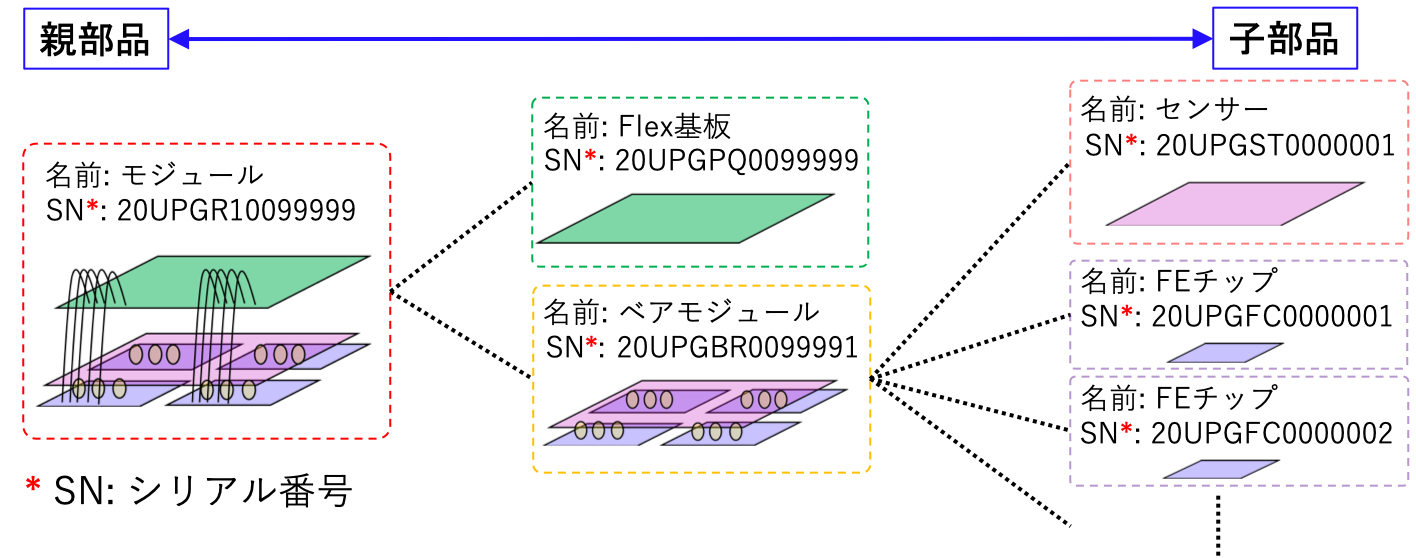
\includegraphics[height=6cm,keepaspectratio]{moduleCP.png}
  \caption[ピクセルモジュールの親子関係]{ピクセルモジュールの親子関係。この図では、Quadモジュールを例にピクセルモジュールの親子関係を示している。}
  \label{fig:moduleCP}
\end{figure}

また、中央データベースではASICが4枚搭載されたQuadモジュールだけではなく、3枚のASICが搭載されているTripletモジュールの情報も取り扱う。Quadモジュールに搭載されるベアモジュールは、センサー1枚とASIC4枚から構成されるのに対して、Tripletモジュールに搭載されるベアモジュールはセンサー1枚とASIC1枚で構成される。また、読み出し試験のテスト用に開発された、センサーが搭載されていないピクセルモジュール(Digitalモジュール)の情報についても中央データベースに登録する。そのため、ピクセルモジュールはいくつかの種類を持ち、それぞれに対して構成するベアモジュールおよびフレキシブル基板の種類が異なる。親子関係を定義する際に、あるピクセルモジュールがどの種類の子部品を持つか定義することにより、データベース上で間違った組み合わせでピクセルモジュールの組み立てをすることを防ぐことができる。あるピクセルモジュールのタイプと組み立て可能なベアモジュールおよびフレキシブル基板の関係を\tref{tab:barepcbtypes}に示す。


\begin{table}[tbp]
  \begin{center}
    \caption[あるピクセルモジュールのタイプと組み立て可能なベアモジュールおよびフレキシブル基板の関係]{あるピクセルモジュールのタイプと組み立て可能なベアモジュールおよびフレキシブル基板の関係。識別IDの項目は、各部品についての種類を識別するためにシリアルナンバーに含まれる4桁の英数字である。}
    \label{tab:barepcbtypes}
    \scalebox{0.9}{
    \begin{tabular}{|l|c||l|c||l|c|}
    \hline
      ベアモジュール & 識別ID & フレキシブル基板 & 識別ID & ピクセルモジュール & 識別ID \\
    \bhline{1.5pt}
      Single bare & PGB1 & Triplet L0 Stave PCB & PIPT & Triplet L0 Stave module & PIMS \\
    \cline{3-6}
      module & & Triplet L0 R0 PCB & PIP0 & Triplet L0 Ring0 module & PIM0 \\
    \cline{3-6}
      &  & Triplet L0 R0.5 PCB & PIP5 & Triplet L0 Ring0.5 module & PIM5 \\
    \hline
      Dual bare & PGB2 & Dual PCB & PGPD & Dual chip module & PGR2 \\
      module & & & & & \\
    \hline
      Quad bare & PGB4 & Quad PCB & PGPQ & L1 quad module & PIM1 \\
      module & & & & & \\
    \cline{5-6}
      &  &  &  & Outer system quad module & PGM2 \\
    \hline
      Digital single & PGBS & Triplet L0 Stave PCB & PIPT & Digital triplet L0 stave module & PIR6 \\
    \cline{3-6}
      bare module &  & Triplet L0 R0 PCB & PIP0 & Digital triplet L0 Ring0 module & PIR7 \\
    \cline{3-6}
      &  & Triplet L0 R0.5 PCB & PIP5 & Digital triplet L0 Ring0.5 module & PIR8 \\
    \hline
      Digital quad & PGBQ & Quad PCB & PGPQ & Digital L1 quad module & PIR9 \\
    \cline{5-6}
      bare module &  &  &  & Digital quad module & PGRB \\
    \hline
      Dummy single & PGBT & Triplet L0 Stave PCB & PIPT & Dummy triplet L0 stave module & PIR3 \\
    \cline{3-6}
      bare module &  & Triplet L0 R0 PCB & PIP0 & Dummy triplet L0 Ring0 module & PIR4 \\
    \cline{3-6}
      &  & Triplet L0 R0.5 PCB & PIP5 & Dummy triplet L0 Ring0.5 module & PIR5 \\
    \hline
      Dummy quad & PGBR & Quad PCB & PGPQ & Dummy L1 quad module & PIR1 \\
    \cline{5-6}
      bare module &  &  &  & Dummy quad module & PGRA \\
    \hline
    \end{tabular}
    }
  \end{center}
\end{table}
%中央データベースにおいて定義されたピクセルモジュールの種類と組み立て可能な子部品の関係を\fref{fig:moduletype}に示す。
%\begin{figure}[tbp]
%  \centering
%  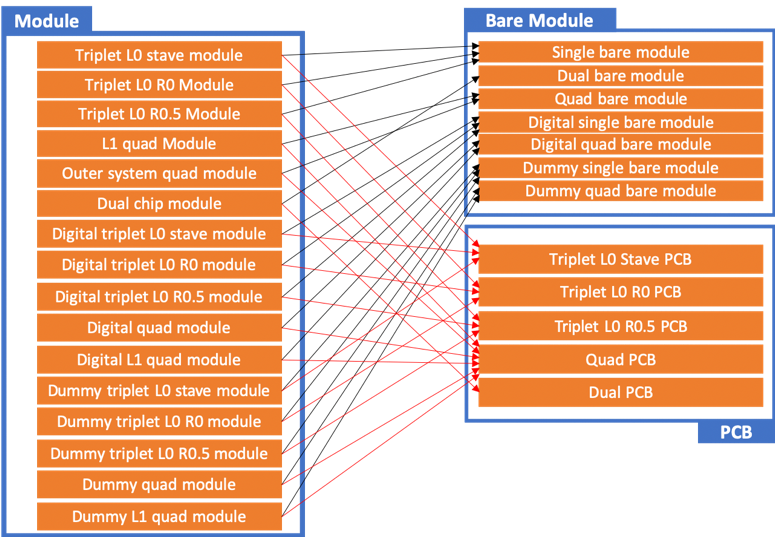
\includegraphics[height=9cm,keepaspectratio]{moduletypes.png}
%  \caption[ピクセルモジュールの種類と組み立て可能な子部品の関係]{ピクセルモジュールの種類と組み立て可能な子部品の関係。}
%  \label{fig:moduletype}
%\end{figure}


ピクセルモジュールはシリアルナンバー(製造番号)を用いて管理される。ITkに搭載されるピクセルモジュールや構成部品に用いられるシリアルナンバーは「20 U xxxx nnnnnnn」のように14桁で定義される。「20」はATLASを構成する部品であることを表し、「U」はITkアップグレードに関連する部品であることを表す。さらに、「xxxx」において各部品の種類の識別を行うことができ、「nnnnnnn」は各部品を特定するための7桁の通し番号である。
さらに、ピクセルモジュールのシリアルナンバーの7桁の通し番号の1桁目はASICの種類を表し、2桁目はセンサーの厚みを表す。通し番号の1桁目、2桁目の数字とASICの種類、センサーの厚みの対応を\tref{tab:serialcomp}に示す。また、ピクセルモジュールとフレキシブル基板は1対1の対応をすることから、最後の5桁はフレキシブル基板と同じになるようにシリアルナンバーが決定される。


\begin{table}[tbp]
  \begin{center}
    \caption[モジュールのシリアルナンバーとASICおよびセンサーの関係]{モジュールのシリアルナンバーとASICおよびセンサーの関係。}
    \label{tab:serialcomp}
    \begin{tabular}{cc}
      \begin{minipage}[tbp]{.45\textwidth}
        \begin{tabular}{|c|c|}
        \hline
          1桁目の数字 & ASICの種類 \\
        \hline
          0 & RD53A \\
          1 & ITkpix\_v1 \\
          2 & ITkpix\_v1.1 \\
          3 & ITkpix\_v2 \\
          9 & No ASIC \\
        \hline
        \end{tabular}
      \end{minipage}
      \begin{minipage}[tbp]{.45\textwidth}
      \begin{tabular}{|c|c|}
        \hline
          2桁目の数字 & センサーの厚み \\
        \hline
          0 & Thin($150\ \si{\micro m}$) \\
          1 & Thick($300\ \si{\micro m}$) \\
        \hline
        \end{tabular}
      \end{minipage}
    \end{tabular}
  \end{center}
\end{table}



%\begin{table}[tbp]
%  \begin{center}
%    \caption[ローカルデータベースのコレクション]{ローカルデータベースのコレクション\cite{oku}}
%    \label{tab:sn}
%    \begin{tabular}{|l||l|}
%    \hline
%      20 & ATLASを構成する検出器を表すコード \\
%    \hline
%      U & ITkアップグレードを表すコード \\
%    \hline
%      xxxx & 各部品の種類を表すコード \\
%    \hline
%      nnnnnnn & 部品を特定するための通し番号 \\
%    \hline
%    \end{tabular}
%  \end{center}
%\end{table}


%------------------------------------------------------------------------------------------------------------------------
\subsubsection{ピクセルモジュール情報の登録機能の開発}
\label{sec:register-module}
%------------------------------------------------------------------------------------------------------------------------

\tref{tab:barepcbtypes}に示したように、中央データベースに定義した構造を用いて、ピクセルモジュール情報を登録する機能の開発を行った。
登録の際に必要な流れは以下の通りである。
\begin{itemize}
  \item[\rnum{1}. ] \tref{tab:barepcbtypes}のように定義されたピクセルモジュールの構造を中央データベースから取得
  \item[\rnum{2}. ] ピクセルモジュールの登録に必要な情報の入力
  \item[\rnum{3}. ] 中央データベースと通信し、ピクセルモジュールを登録および構成部品を登録
\end{itemize}

\subsubsection{\rnum{1}. ピクセルモジュールの構造を中央データベースから取得}

ピクセルモジュールを中央データベースに登録する際、\tref{tab:barepcbtypes}に示されている組み合わせに基づいて構成部品の情報を登録する必要がある。ローカルデータベースのウェブブラウザからピクセルモジュールの登録を行うために、登録するピクセルモジュールの種類に対して、適切な種類のベアモジュールおよびフレキシブル基板が使用されているかを確認する必要がある。

ローカルデータベースにおいて、適切な種類のベアモジュールとフレキシブル基板が使用されていることを確認するために、Code\ref{code:childParentRelation}に示すドキュメントをQC.module.typesのコレクションに作成する。
\cref{code:childParentRelation}は中央データベースからピクセルモジュールの構造についてのデータをダウンロードし、必要な情報を抽出することにより作成される。このドキュメントは全てのピクセルモジュールについて共通のドキュメントであり、他組み立て機関においても同様の構造を持つことから、 QC.module.typesはlocaldbtoolsのデータベースにおいて管理する。\cref{code:childParentRelation}は以下の情報を保持する。ここで、以下の括弧内は\cref{code:childParentRelation}におけるキー値を表している。
\begin{itemize}
  \item ドキュメント作成時のデータベースのバージョン情報(dbVersion)
  \item ピクセルモジュールをITkに実装する際の大まかな位置情報(subprojects)
  \item ピクセルモジュールの種類と識別コード(types)
  \item ピクセルモジュールの子部品情報(children)
\end{itemize}

\begin{lstlisting}[caption=ピクセルモジュールの組み立て工程を管理するためのドキュメントの一部。,label=code:childParentRelation, language=C++]
{
  "_id" : ObjectId("5bb1e1bef981520009c54bc5"),
  "dbVersion" : 1.01,
  "code" : "MODULE",
  "name" : "Module",
  "project" : {
    "code" : "P",
    "name" : "Pixels"
  },
  "subprojects" : [
    {
      "code" : "PI",
      "name" : "Inner pixels"
    },
    {
      "code" : "PB",
      "name" : "Outer pixel barrel"
    },
    {
      "code" : "PE",
      "name" : "Pixel endcaps"
    },
    {
      "code" : "PG",
      "name" : "Pixel general"
    }
  ],
  "types" : [
    {
      "code" : "TRIPLET_L0_STAVE_MODULE",
      "name" : "Triplet L0 stave module",
      "subprojects" : [
        {
          "code" : "PI",
          "name" : "Inner pixels"
        }
      ],
      "snComponentIdentifier" : "MS"
    },
    ...
  ],
  "children" : {
  "TRIPLET_L0_STAVE_MODULE" : {
	  "BARE_MODULE" : "PGB1",
	  "PCB" : "PIPT"
  },
    ...
  }
}
\end{lstlisting}

\subsubsection{\rnum{2}. ピクセルモジュールの登録に必要な情報の入力}

ピクセルモジュールを中央データベースに登録する際に入力必須情報を\tref{tab:nyuuryoku}に示す。
ピクセルモジュールを登録する際には、これらの情報を中央データベースに送信する必要があるが、入力項目が多いことから入力ミスが発生する可能性ある。一般的に人がルーティーンタスクにおいて入力ミスをする確率は$0.3\%$であることが知られている\cite{human}。各ピクセルモジュールに必要な入力項目は$11$項目であり、日本においてはこの作業を約$2200$回(ピクセルモジュールの数)繰り返すため、最大$60$個程度のピクセルモジュールに対して誤った情報が記録されてしまうと予想される。
さらに、\tref{tab:nyuuryoku}に示した入力情報は、データベースの構造を熟知した人であれば項目から入力する内容を直ちに理解することができるが、品質試験を行う試験者はデータベースについて詳しいとは限らない。

\begin{table}[tbp]
  \begin{center}
    \caption[ピクセルモジュール登録に必要な入力情報]{ピクセルモジュール登録に必要な入力情報}
    \label{tab:nyuuryoku}
    \begin{tabular}{|l||l|l|}
    \hline
    & project &  ピクセルモジュールの場合は"P"を入力 \\
    \cline{2-3}
    & subproject & ITkに搭載する際の大まかな位置情報 \\
    \cline{2-3}
    ピクセルモジュール
    & institution & 登録者の所属機関 \\
    \cline{2-3}
    基本情報
    & componentType & ピクセルモジュールの場合は"MODULE"を入力 \\
    \cline{2-3}
    & type & ピクセルモジュールの種類 \\
    \cline{2-3}
    & ATLAS Serial Number & 14桁のシリアルナンバー \\
    \hline
    ピクセルモジュール
    & FE chip version & 搭載されるASICの種類 \\
    \cline{2-3}
    特性情報 & Thickness & 搭載されるセンサーの厚み情報 \\
    \hline
    組み立て部品 & ベアモジュール & 14桁のシリアルナンバー \\
    \cline{2-3}
    情報 & フレキシブル基板 & 14桁のシリアルナンバー \\
    \cline{2-3}
     & モジュールキャリア & 14桁のシリアルナンバー \\
    \hline
    \end{tabular}
  \end{center}
\end{table}

そこで、ローカルデータベースにおけるピクセルモジュールの登録機能では、入力ミスを防ぐために入力パラメータを必要最低限に削減し、入力フォーマットを簡略化するように設計した。入力パラメータを削減するために、別のパラメータから情報を抽出する手法を導入した。ピクセルモジュール登録のための入力パラメータと削減したパラメータを以下に示す。
\begin{itemize}
  \item 入力パラメータ
  \begin{itemize}
    \item ピクセルモジュールの種類情報
    \item ベアモジュールのシリアルナンバー
    \item フレキシブル基板のシリアルナンバー
    \item モジュールキャリアのシリアルナンバー
  \end{itemize}
  \item 削減したパラメータ
  \begin{itemize}
  \item project: 本機能ではピクセルモジュールのみであるから"P"で固定
  \item subproject: ピクセルモジュールの種類情報から抽出
  \item institution: 中央データベースにアクセスする際のユーザー情報から抽出
  \item componentType: 本機能ではピクセルモジュールのみであるから"MODULE"で固定
  \item ATLAS Serial Number: ベアモジュールおよびフレキシブル基板のシリアルナンバーから自動生成
  \item FE chip version: ベアモジュール情報から抽出
  \item Thickness: ベアモジュール情報から抽出
  \end{itemize}
\end{itemize}

この手法を導入することにより、ピクセルモジュールの登録の際に必要な入力パラメータを半数以下に減らすことができる。ローカルデータベースのウェブページにおけるピクセルモジュールの登録画面を\fref{fig:module-touroku-gamen}に示す。入力ミスを防ぐために、ピクセルモジュールの種類はプルダウンから選択するようにし、各部品のシリアルナンバーを入力する欄は、14桁の英数字のみ入力できるものとした。

\begin{figure}[tbp]
  \centering
  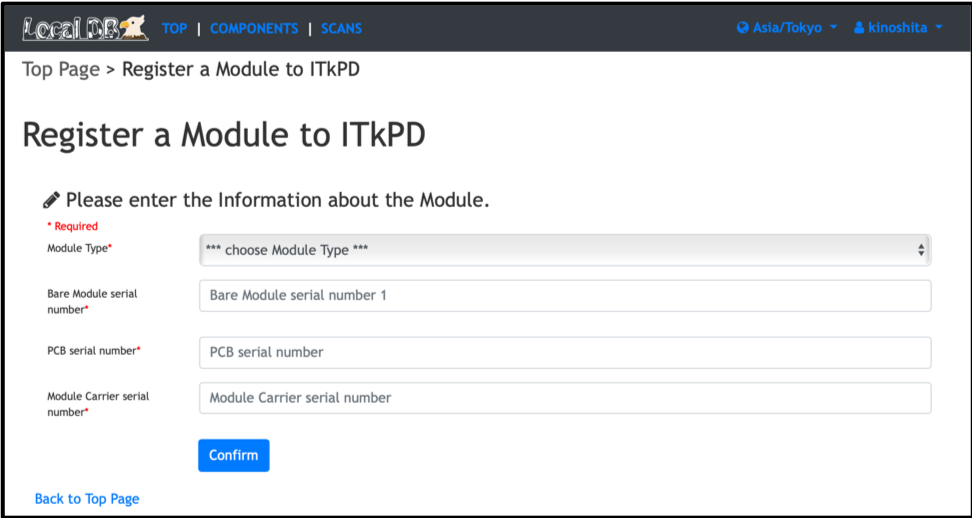
\includegraphics[height=7cm,keepaspectratio]{moduletouroku.png}
  \caption[ローカルデータベースを用いたピクセルモジュール登録画面]{ローカルデータベースを用いたピクセルモジュール登録画面。}
  \label{fig:module-touroku-gamen}
\end{figure}

また、Tripletモジュールはフレキシブル基板1枚とベアモジュール3つから構成される。そのため、\fref{fig:module-touroku-gamen}に示したピクセルモジュール登録画面において、Tripletモジュールである種類のモジュールが選択された場合には、ベアモジュールについての入力欄を3つに増やすようにした。

\subsubsection{\rnum{3}. 中央データベースと通信し、ピクセルモジュールを登録および構成部品を登録}

入力した情報を用いて中央データベースと通信し、ピクセルモジュールの登録およびデータベース上において構成部品の組み立てを行う。\fref{fig:dbregistermodule}にピクセルモジュール登録機能による処理の流れを示す。\fref{fig:module-touroku-gamen}において入力した情報と、中央データベースへのログインパスワードを用いてピクセルモジュールの登録を行う。登録の際に、各部品が中央データベース上に存在すること、データベース上で組み立て可能であることを確認する。これにより、本来とは異なる部品によるピクセルモジュールの登録を一部防ぐことができる。

\begin{figure}[tbp]
  \centering
  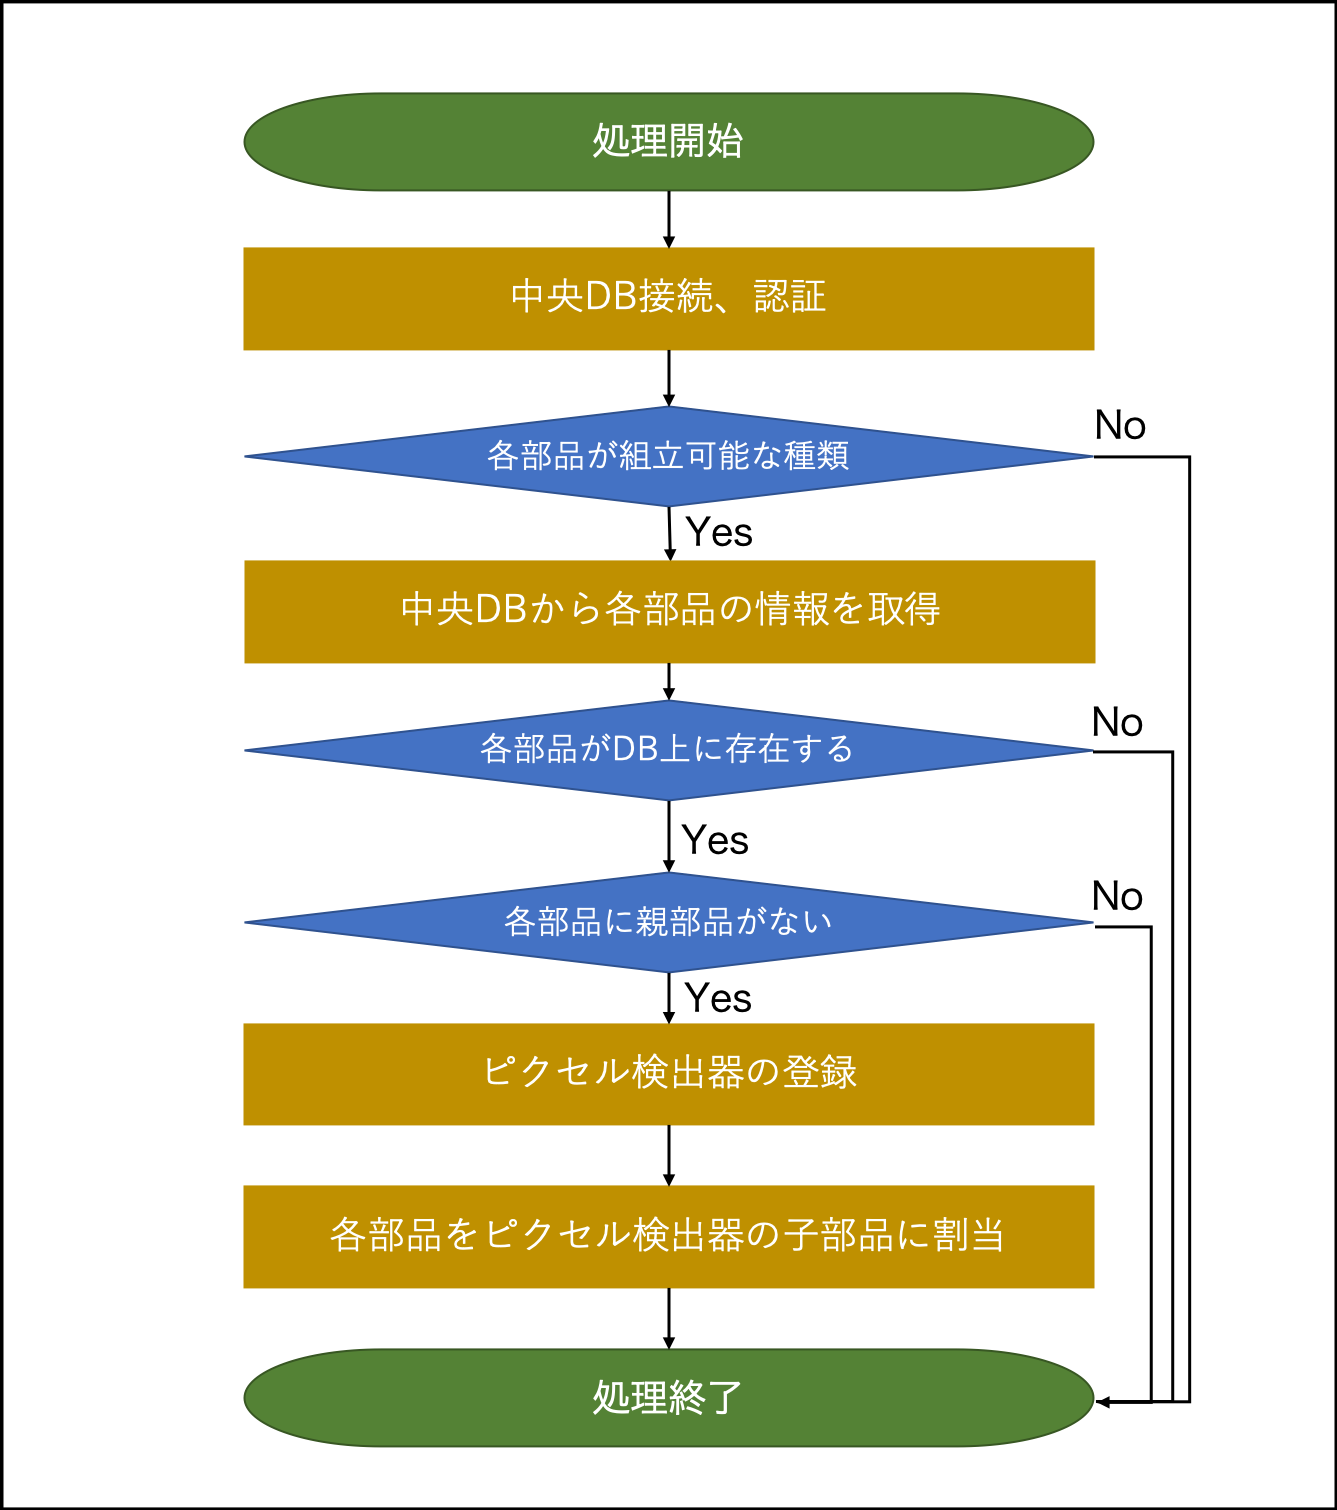
\includegraphics[height=10cm,keepaspectratio]{registerflow.png}
  \caption[ピクセルモジュール登録機能による処理の流れ]{ピクセルモジュール登録機能による処理の流れ。}
  \label{fig:dbregistermodule}
\end{figure}


%------------------------------------------------------------------------------------------------------------------------
\subsection{品質試験結果の同期機能}
\label{sec:upload-result}
%------------------------------------------------------------------------------------------------------------------------

第\ref{sec:chap6}で示したように、ピクセルモジュールを複数機関で組み立てを行う場合や、品質試験を終えてCERNに送った際に、ピクセルモジュールの受け取り先の機関において輸送中にピクセルモジュールに損傷がないことを確認するため、品質管理試験を行う。そのために、輸送前後の品質試験結果を比較することや輸送前の設定値を用いて読み出し試験を行う必要がある。

本研究において、先行研究\cite{oku}で開発された読み出し試験結果を中央データベースにアップロードする機能を拡張し、全ての品質管理試験結果およびピクセルモジュールの組み立て工程を中央データベースと同期する機能の開発を行った。


\subsubsection{中央データベースにおける品質試験結果の管理方法}

先行研究において、中央データベースにおけるピクセルモジュールの組み立て工程と付随する品質管理試験項目の実装が行われた。
各品質試験項目について、アップロードする情報を以下に示す。
\begin{itemize}
  \item ピクセルモジュールのシリアルナンバー
  \item 試験日時
  \item 試験機関
  \item コメント
  \item ローカルデータベースを再現するためのファイル
  \item[※] 品質試験結果
  \item[※] 品質試験特性
\end{itemize}
上記において、「・」で記した情報は全ての試験項目において共通であり、「※」で記した情報は各試験項目で固有の値を持つ。ローカルデータベースはNoSQLのMongoDBを用いて品質試験結果を管理しているため、品質試験結果に含まれるパラメータを定義することなく柔軟に管理できるが、中央データベースにおいては各試験項目について、アップロードするパラメータの枠を定義し、その枠に従った形の情報のみを管理することができる。非読み出し試験について、中央データベースに定義したアップロードするパラメータの枠を\tref{tab:resultpara}に示す。

\begin{table}[tbp]
  \begin{center}
    \caption[中央データベースに定義したパラメータ]{中央データベースに定義したアップロードパラメータ}
    \label{tab:resultpara}
    \begin{tabular}{|l||c|l|c|}
    \hline
      品質試験項目 & 種類 & パラメータの種類 & パラメータのタイプ \\
    \bhline{1.5pt}
      \multirow{2}{*}{質量測定}
      & 結果 & 質量 & float \\
    \cline{2-4}
      & 特性 & 測定精度 & float \\
    \hline
      \multirow{1}{*}{質量測定}
      & 結果 & 全体画像 & image \\
    \hline
      \multirow{1}{*}{平坦性測定}
      & 結果 & 平坦性測定結果 & 1次元のlist \\
    \hline
      \multirow{7}{*}{センサーIV特性}
      & 結果 & 電流値 & 1次元のlist \\
      &  & 電流の分散値 & 1次元のlist \\
      &  & 電圧 & 1次元のlist \\
      &  & 温度 & 1次元のlist \\
      &  & 湿度 & 1次元のlist \\
      &  & 時間 & 1次元のlist \\
    \cline{2-4}
      & 特性 & 室温 & float \\
    \hline
      \multirow{7}{*}{SLDO VI特性}
      & 結果 & 電流値 & 1次元のlist \\
      &  & 電圧 & 1次元のlist \\
      &  & 電圧の分散値 & 1次元のlist \\
      &  & 温度 & 1次元のlist \\
      &  & 湿度 & 1次元のlist \\
      &  & 時間 & 1次元のlist \\
    \cline{2-4}
      & 特性 & 室温 & float \\
    \hline
      \multirow{10}{*}{ワイヤボンド強度測定}
      & 結果 & 平均負荷値 & float \\
      &  & 負荷の分散値 & float \\
      &  & 最大負荷値 & float \\
      &  & 最小負荷値 & float \\
      &  & ワイヤボンド部の損傷割合 & float \\
    \cline{2-4}
      & 特性 & 使用した機械の名前 & string \\
      &  & 試験者の名前 & string \\
      &  & テストのスピード & float \\
      &  & ボンド部の高さ & float \\
      &  & 負荷のテスト値 & float \\
    \hline
      \multirow{7}{*}{ワイヤボンド情報}
      & 結果 & 温度 & float \\
      &  & 湿度 & float \\
    \cline{2-4}
      & 特性 & 使用した機械の名前 & string \\
      &  & 試験者の名前 & string \\
      &  & ワイヤーボンドに用いたジグ & string \\
      &  & ワイヤーボンドのプログラム & string \\
      &  & ワイヤーボンドのバッチ数 & string \\
    \hline
      & 結果 & 室温 & float \\
      ベアモジュールと &  & 湿度 & float \\
    \cline{2-4}
      フレキシブル基板の& 特性 & 接着剤の比率 & float \\
      接着情報&  & バッチナンバー & string \\
      &  & 試験者の名前 & string \\
      &  & 接着方法 & string \\
    \hline
    \end{tabular}
  \end{center}
\end{table}


\subsubsection{品質試験結果のアップロード機能}

\tref{tab:resultpara}のように中央データベースに定義した品質試験のパラメータを用いて、品質試験結果をアップロードする機能の開発を行った。
各品質試験結果をアップロードするための処理を以下に示す。
\begin{itemize}
  \item[1. ] 中央データベースからアップロードするパラメータの枠を取得
  \item[2. ] ローカルデータベースから試験結果を抽出し、各パラメータの枠に値を埋める
  \item[3. ] 作成した結果を中央データベースへアップロード
  \item[4. ] アップロードした結果にデータファイルを添付
\end{itemize}
4番目の処理の際に、読み出し試験における試験結果のJSON fileや外観検査についての画像ファイルの添付を行う。さらに、ローカルデータベースの各品質試験結果を表すドキュメントについてもJSONファイルに変換し添付する。このJSONファイルをダウンロードすることにより、別の組み立て機関に設置したローカルデータベースにおいて試験結果の再現を行うことができるよう設計した。

中央データベースは各組み立て機関において保存されている全ての結果を保存するのではなく、ある組み立て工程におる本結果のみを中央データベースに同期する。ある組み立て工程において、本結果を選択する機能において選ばれた結果を一括アップロードする機能の開発を行った。
品質試験結果のアップロード処理の流れを\fref{fig:uploadresults}に示す。この処理の流れのループに示すように、選択機能を用いて選択された品質試験結果を中央データベースへ一括アップロードを行う。さらに、アップロード処理を行っている工程がワイヤー配線であれば、ピクセルモジュールの特性項目のアップロード処理も行う。
ループ中の条件分岐において、同一の試験結果が中央データベースにアップロードされていないかの確認を行う。これにより、中央データベースにおいて結果の重複を避けることができる。

ローカルデータベースにおいて、複数の組み立て工程において試験結果の選択が行われている場合は、アップロード処理を繰り返す。これを繰り返すことにより、最終的にローカルデータベースにおけるピクセルモジュールの組み立て工程の一つ前の工程までの品質試験結果のアップロード処理を行う。各ループの最後に、中央データベースの組み立て工程を一つ後の工程に変更するため、最終的にローカルデータベースと中央データベースの組み立て工程が同一のものとなり、ピクセルモジュールの組み立て工程の情報の同期を行うことができる。よって、中央データベースにおいてピクセルモジュールの量産過程が実際に行われている各組み立て機関の進捗度と同じになり、中央データベースにおけるデータを確認すれば、量産の進捗度を確認することができる。

\begin{figure}[tbp]
  \centering
  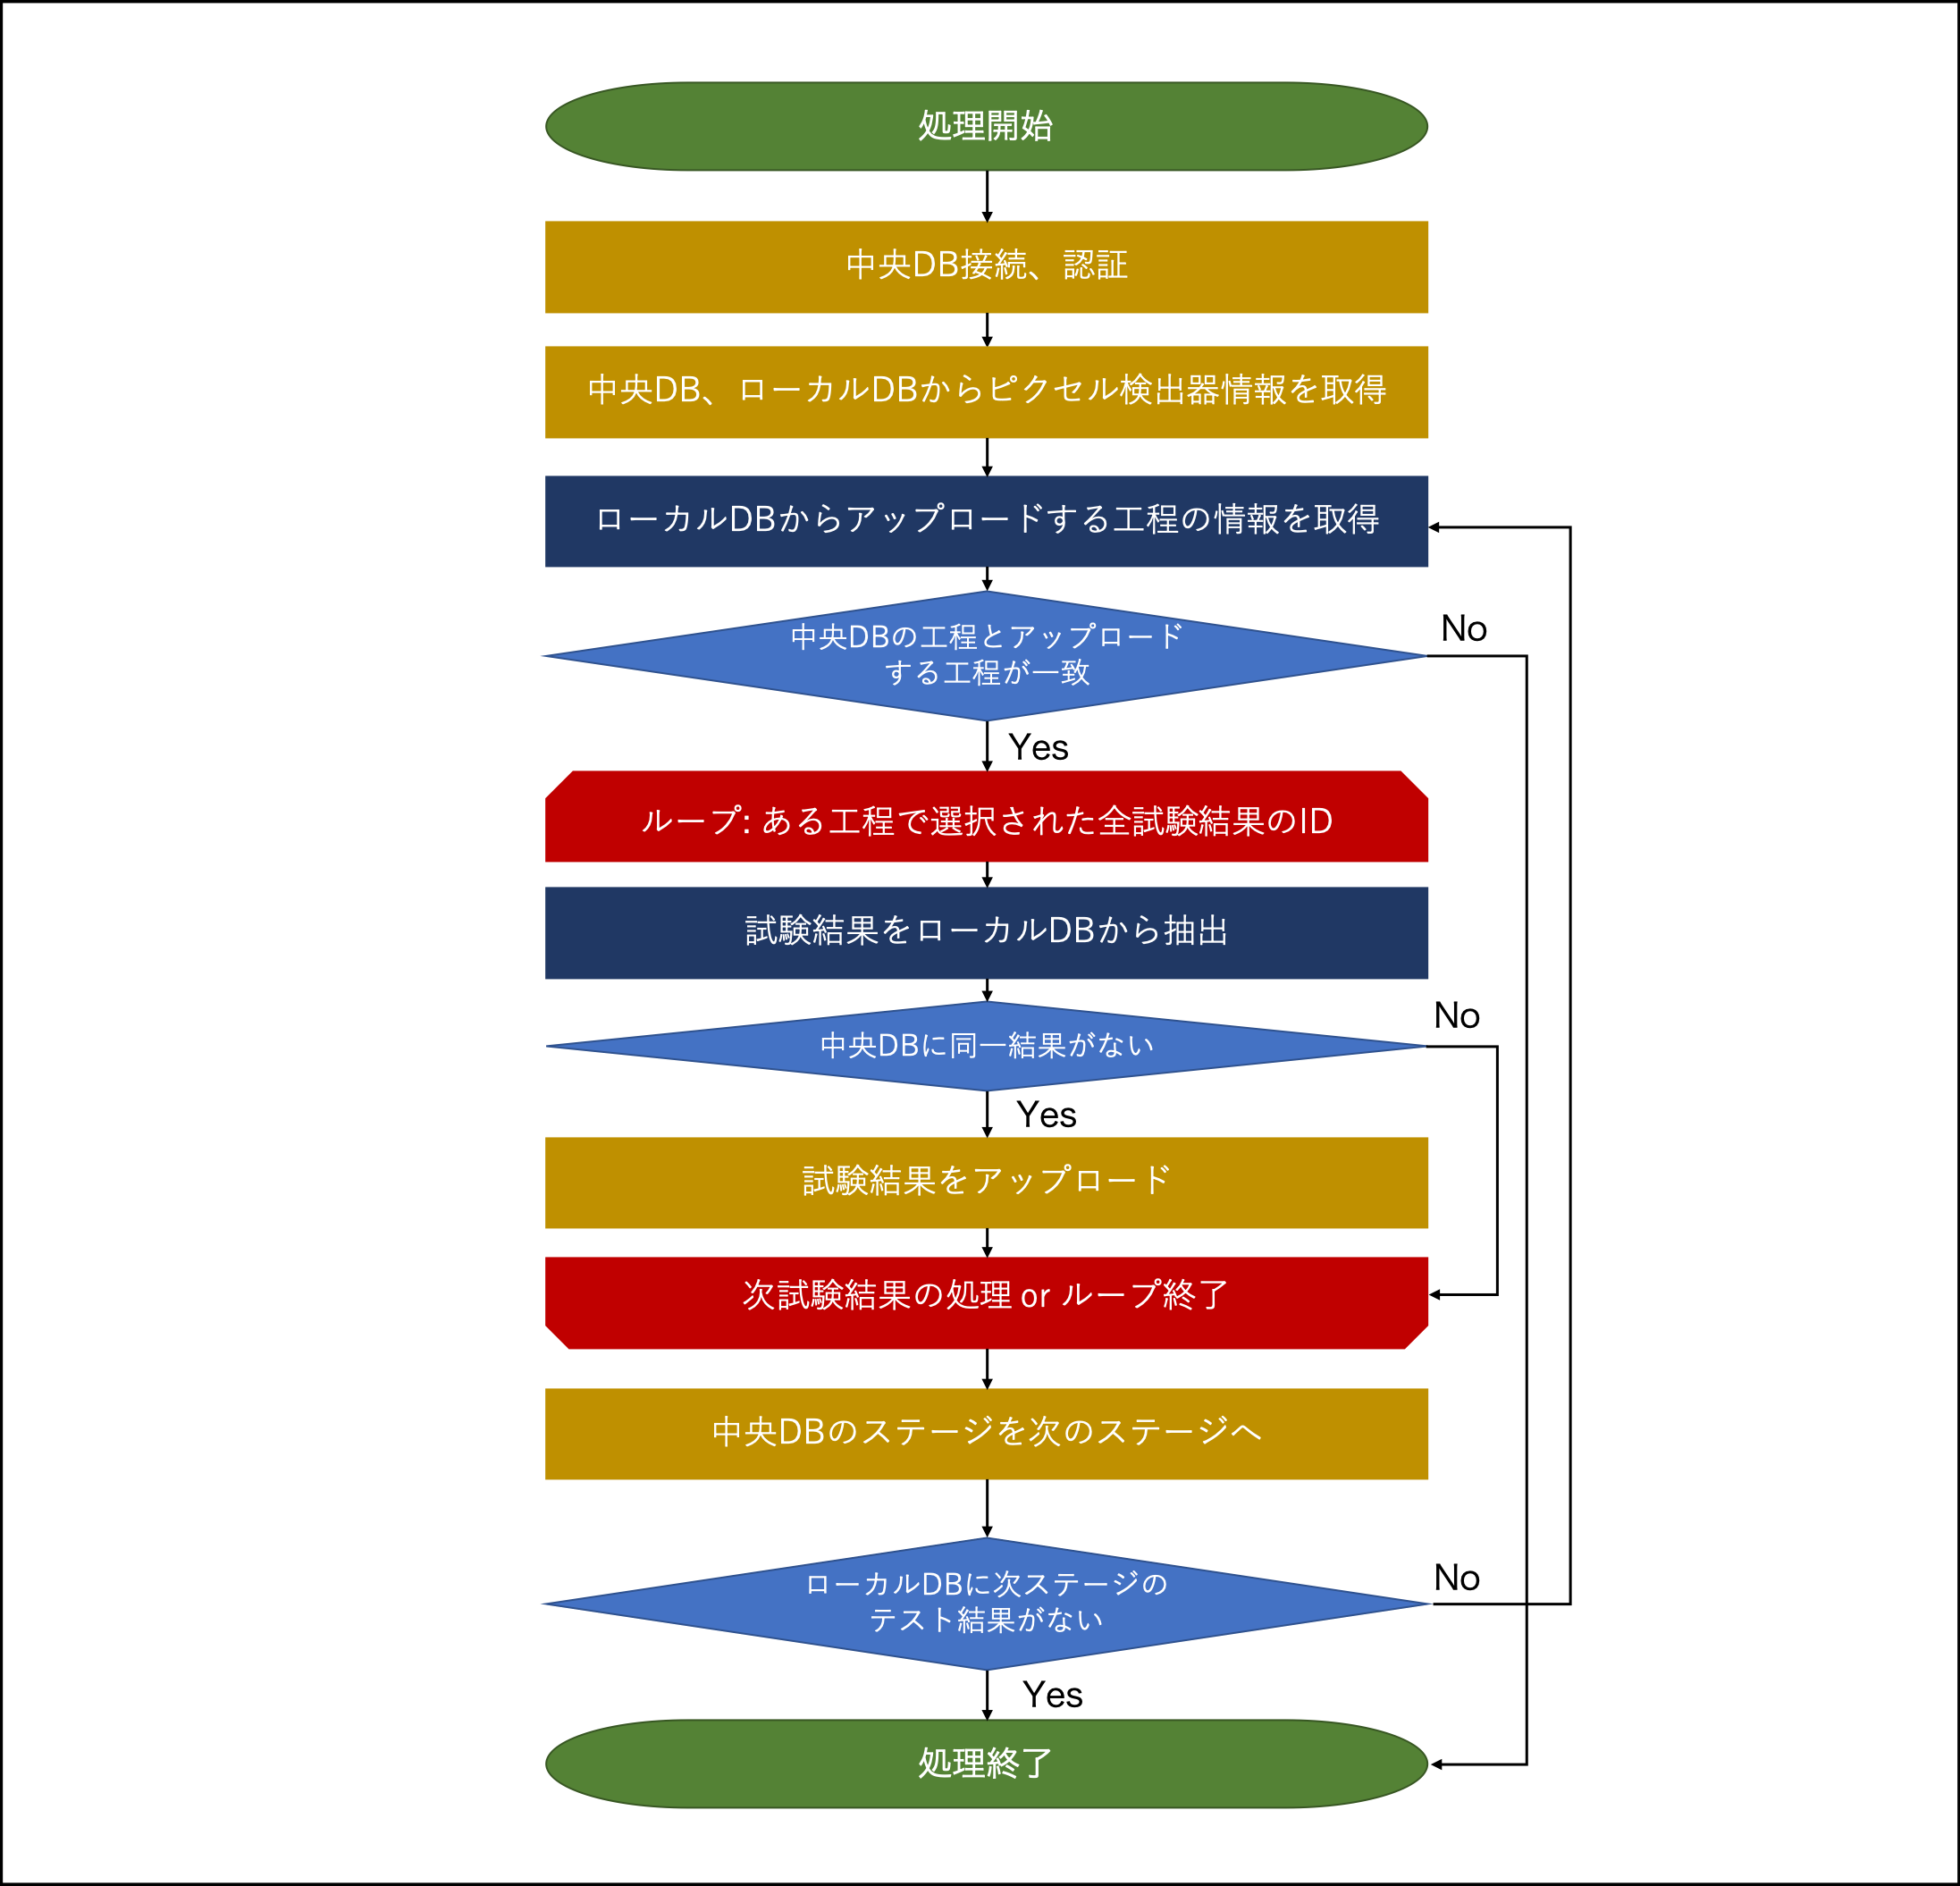
\includegraphics[height=14cm,keepaspectratio]{uploadflow.png}
  \caption[品質試験結果アップロード処理の流れ]{品質試験結果アップロード処理の流れ。}
  \label{fig:uploadresults}
\end{figure}


\subsubsection{アップロード機能の性能評価}

開発した機能の実用性を検証するためにアップロード機能の性能評価を行った。実際の組み立て機関で用いるハードウェアに近い環境で行うために、自身のラップトップ環境ではなく、陣内研究室で管理しているサーバーを用いて性能評価を行った。サーバーのCPUはIntel Core i3 2.93GHz、通信速度は$47.5\ \si{MB/sec}$\footnote{測定を行った2021年9月時の値}である。

測定方法として、以下の処理100回繰り返し、その平均を処理時間とし分散を誤差導出した。
\begin{itemize}
  \item[1. ] 品質試験結果を表すIDを用いて試験結果をローカルDBから抽出
  \item[2. ] 品質試験結果を中央データベースへアップロード
\end{itemize}
アップロード機能の性能評価結果を\tref{tab:sokuteikekka}に示す。

\begin{table}[tbp]
  \begin{center}
    \caption[アップロード機能の処理時間の測定結果]{アップロード機能の処理時間の測定結果}
    \label{tab:sokuteikekka}
    \begin{tabular}{|l||c|l|r|}
    \hline
      品質試験項目 & データ形式 & 容量 & 処理時間 \\
    \bhline{1.5pt}
      質量測定 & テキスト & $8\ \si{B}$ & $1.9\pm0.7\ [\si{sec}]$ \\
    \hline
      平坦性測定 & テキスト & $88\ \si{B}$ & $2.0\pm0.5\ [\si{sec}]$ \\
    \hline
      外観検査 & 画像(png) & $3.7\ \si{MB}$ & $8.8\pm3.9\ [\si{sec}]$ \\
    \hline
      読み出し試験 & zipファイル & $3.9\ \si{MB}$ & $161.4\pm10.0\ [\si{sec}]$ \\
    \hline
    \end{tabular}
  \end{center}
\end{table}

読み出し試験のアップロードにかかる処理時間は$\mathcal{O}(100)$であり、読み出し試験以外の結果については処理時間が$\mathcal{O}(1)$となった。1つの工程に定義される読み出し試験以外の品質試験は最大7項目であるため$20$秒程度で処理が終わり、実用可能だと考えられる。しかし、読み出し試験についてはアップロード処理に5分以上処理時間を要する。中央データベースへのアップロード処理は、ウェブブラウザのボタンを押せば\fref{fig:uploadresults}の流れに沿って自動で処理を行うため、休憩時間の前などに行えば実用可能であると考えられるが、アップロード処理中にネットワークが不安定になるようなことが起きると途中で処理が止まり、不十分なデータが中央データベースに残ってしまう。処理時間が長くなる原因としては以下の2つが挙げられる。
\begin{itemize}
  \item アップロードの処理に用いる中央データベースとの通信APIの処理時間
  \item ローカルデータベースから試験結果を抽出するのにかかる処理時間
\end{itemize}

初めに中央データベースとの通信APIの処理時間について考察する。各品質試験結果をアップロードする際に使用するAPIの一覧を\tref{tab:uploadapi}に示す。非読み出し試験の場合は、「generateTestTypeDtoSample」、「uploadTestRunResults」をそれぞれ1回行い、「createTestRunAttachment」を1回(ローカルデータベースを再現するためのJSONファイル)$+$添付するデータファイルの数だけ行う。アップロードするデータの容量は通信速度$47.5\ [\si{MB/sec}]$と比較して小さいため、APIの使用回数に処理時間が律速されると考えられる。


\begin{table}[tbp]
  \begin{center}
    \caption[アップロード機能に使用されるAPI一覧]{アップロード機能に使用されるAPI一覧}
    \label{tab:uploadapi}
    \begin{tabular}{|l||l|r|}
    \hline
      関数名 & 処理の内容 & 処理時間の平均 \\
    \bhline{1.5pt}
      generateTestTypeDtoSample & \tref{tab:resultpara}に定義した情報を取得 & $0.65 \pm 0.43\ [\si{sec}]$ \\
    \hline
      uploadTestRunResults & 品質試験結果を登録 & $0.88 \pm 0.55\ [\si{sec}]$ \\
    \hline
      createTestRunAttachment & 試験結果にデータファイルを添付 & $0.60 \pm 0.17 \ [\si{sec}]$ \\
    \hline
    \end{tabular}
  \end{center}
\end{table}

一方で、読み出し試験はピクセルモジュールのみではなく、各ASICについても結果が作成される。そのため、クアッドモジュールの場合は「generateTestTypeDtoSample」、「uploadTestRunResults」をそれぞれ5回行い、「createTestRunAttachment」は34回行う。そのため、APIを用いた場合の処理時間は\eref{eq:elecshori}のようになる。
\begin{equation}
  \label{eq:elecshori}
  (0.65 \pm 0.43) \times 5 + (0.88 \pm 0.55) \times 5 + (0.60 \pm 0.17) \times 34 \simeq 28.05 \pm 1.81 \ [\si{sec}]
\end{equation}
ここで、アップロードするデータの容量は通信速度$47.5\ [\si{MB/sec}]$と比較して小さく無視できるものとし、\tref{tab:uploadapi}に示したものと同程度になると仮定して計算を進めた。\fref{eq:elecshori}より、中央データベースとの通信にかかる処理時間は$30$秒程度であるが、\tref{tab:sokuteikekka}で求められた処理時間はこれに比べて非常に長くなっている。そのため、ローカルデータベースから読み出し試験結果を抽出する際の処理時間が原因でアップロード処理に時間を要していると考えられる。

ローカルデータベースからの読み出し試験結果の抽出処理は、先行研究\cite{kubotan}によって開発されたダウンロードツールを用いている。ダウンロードツールを用いて読み出し試験結果を抽出する際に要する処理時間を\tref{tab:elecdownload}に示す。これにより、読み出し試験結果の抽出に$79$秒かかることがわかる。さらに、抽出したデータはZIPファイルに圧縮された後に、中央データベースにおける品質試験結果に添付される。圧縮処理の平均時間は$0.26 \pm 0.21\ [\si{sec}]$であり、作成するZIPファイルは34個である。そのため、ローカルデータベースにおいて中央データベースにアップロードする読み出し試験結果の作成のために、$90$秒程度の処理時間を要する。

%\begin{figure}[tbp]
%  \centering
%  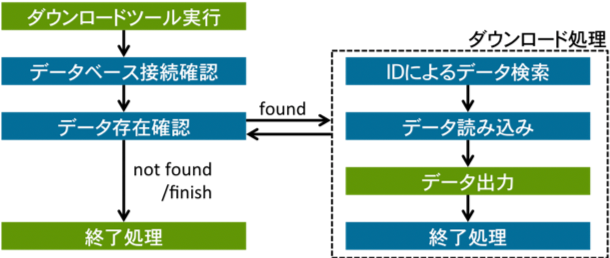
\includegraphics[height=5cm,keepaspectratio]{downloadtool.png}
%  \caption[ダウンロードツールの概念図]{ダウンロードツールの概念図\cite{kubotan}。}
%  \label{fig:elecpull}
%\end{figure}

\begin{table}[tbp]
  \begin{center}
    \caption[ダウンロードツールの処理時間]{ダウンロードツールの処理時間}
    \label{tab:elecdownload}
    \begin{tabular}{|l||r|r|}
    \hline
      スキャン項目 & 抽出するデータファイル数 & 処理時間の平均 \\
    \bhline{1.5pt}
      デジタルスキャン & 31 (96.8 MB) & $11.36 \pm 1.15\ [\si{sec}]$ \\
    \hline
      アナログスキャン & 31 (96.8 MB) & $9.21 \pm 1.11\ [\si{sec}]$ \\
    \hline
      スレッショルドスキャン & 204 (118.6 MB) & $11.13 \pm 0.91\ [\si{sec}]$ \\
    \hline
      ToTスキャン & 47 (112.9 MB)& $10.12 \pm 1.27\ [\si{sec}]$ \\
    \hline
      ノイズスキャン & 31 (102.8 MB) & $9.05 \pm 0.75\ [\si{sec}]$ \\
    \hline
      クロストークスキャン & 161 (272.8 MB) & $28.08 \pm 2.61\ [\si{sec}]$ \\
    \hline
    \hline
      合計 & 505 (800.7 MB) & $78.95 \pm 3.52 \ [\si{sec}]$ \\
    \hline
    \end{tabular}
  \end{center}
\end{table}


\subsubsection{アップロード処理時間の改善案}

\fref{fig:uploadresults}に示した流れでアップロード処理を行うと、読み出し試験を含む工程では$2$分以上かかってしまう。ブラウザの応答に時間がかかると、使用者の満足感や信頼感の低下の原因となり、ユーザーエクスペリエンスが非常に悪くなる。
そこで、本研究においてはバックグラウンドでアップロード処理を行うことにし、使用者のブラウザ応答待機時間を削減させた。使用者がアップロード開始のボタンを押した後、中央データベースへの接続およびユーザー認証を完了した後、バックグランド処理を行うようにした。これにより、使用者の待ち時間は接続およびユーザー認証にかかる$3.10 \pm 0.38\ [\si{sec}]$\footnote{中央データベースへの接続およびユーザー認証処理を$100$回行い、その平均と分散を計算した。}となり、待ち時間を抑えることができた。

バックグラウンドで処理を行うと、ネットワークの接続切れやアップロード機能のバグが原因で処理が中断されても使用者が問題に気づかないということが発生する。そのような問題を防ぐため、品質試験結果アップロードのバックグラウンド処理が中断された時にブラウザ上に問題を表示する機能の実装を行った。

バックグラウンド処理により、ブラウザの応答時間は短縮できるが、実際に行う処理時間に変化はないため、今後この改善を行う必要がある。
中央データベースとの通信を伴う処理は、中央データベースAPI開発者によるものであるため、本研究の対象外である。今後改善可能な処理を以下に示す。
\begin{itemize}
  \item[1. ] 添付するデータファイルの数の削減
  \item[2. ] ローカルデータベースからデータを抽出する処理時間の削減
\end{itemize}

項目1に関して、読み出し試験における品質試験に添付するデータファイルの数は34個である。読み出し試験はピクセルモジュールのみではなく、各ASIC毎に作成され、結果添付ファイルは、読み出し試験における6項目のスキャンについて作成される。データファイルを添付するための関数は"createTestRunAttachment"であり、\tref{tab:uploadapi}から、この通信の処理に$20.4 \pm 0.99\ [\si{sec}]$だけ必要となる。そこで、圧縮するファイルの数を変更しデータファイルの添付を行い、その処理時間の変化を確認した。ファイルの圧縮方法として以下の2つについて考える。
\begin{itemize}
  \item 全てのデータファイルを一つのZIPファイルにまとめる
  \item ピクセルモジュールおよび各ASICに対するデータファイルをそれぞれ一つのZIPファイルにまとめる
\end{itemize}
これらの処理時間の測定結果を\tref{tab:asshuku}に示す。

\begin{table}[tbp]
  \begin{center}
    \caption[アップロード機能に使用されるAPI一覧]{アップロード機能に使用されるAPI一覧}
    \label{tab:asshuku}
    \begin{tabular}{|l||l|r|}
    \hline
      まとめ方 & ZIPファイルの容量 & 処理時間の平均 \\
    \bhline{1.5pt}
      全ての結果 & $10\ \si{MB}$ & \multicolumn{1}{c|}{-} \\
    \hline
      ピクセルモジュール & $ 29\ \si{KB} $ & $0.88 \pm 0.8\ [\si{sec}]$ \\
    \hline
      1つのASIC & $2.5\ \si{MB}$ & $4.30 \pm 0.94 \ [\si{sec}]$ \\
    \hline
    \end{tabular}
  \end{center}
\end{table}

全ての結果をまとめた場合はエラーが発生し添付に失敗した。これは、データファイルを添付するための関数"createTestRunAttachment"は$4\ \si{MB}$以上のデータを扱えないことが原因である。よって、今回確認した中で可能な添付の処理方法は、ピクセルモジュールと各ASICの結果をそれぞれまとる方法のみであり、処理時間は\eref{eq:asshuku}となる。
\begin{equation}
  \label{eq:asshuku}
  (0.88 \pm 0.8) + 4\times(4.30 \pm 0.94) = 18.8 \pm 2.04\ [\si{sec}]
\end{equation}
\eref{eq:asshuku}から得られる結果は$20.4 \pm 0.99\ [\si{sec}]$と比較して大きな改善は期待できない。

項目2に関して、マルチスレッドを用いて、各試験項目抽出処理の並列化をすることにより抽出処理にかかる時間を削減することが考えられる。\tref{tab:elecdownload}からそれぞれのスキャン項目について、ローカルデータベースから結果を取得することに10秒程度かかっていることがわかる。この抽出処理を並列化することにより、処理時間が削減でき、最も時間のかかるクロストークスキャンについての時間に律速され、処理時間を$50$秒程度削減できると考えられる。


\subsubsection{品質試験結果のダウンロード機能}


\fref{fig:downloadresults}に品質試験結果のダウンロード機能の全体像を示す。中央データベースに添付した品質試験結果のドキュメント情報を保有するJSONファイルをダウンロードすることにより同期を行う。このJSONファイルには、品質試験結果を識別するためのオブジェクトIDが記述されている。同一オブジェクトIDの品質試験結果がQC.resultsのコレクション内に存在するかを確認することにより、品質結果の重複を避けることができる。

さらに、全ての品質試験結果のダウンロード処理の後に、中央データベースにおけるピクセルモジュールの組み立て工程をローカルデータベースへ同期する。これにより、ピクセルモジュールを輸送した後、受け取り機関において正しい組み立て工程における品質管理を行うことができる。

\begin{figure}[tbp]
  \centering
  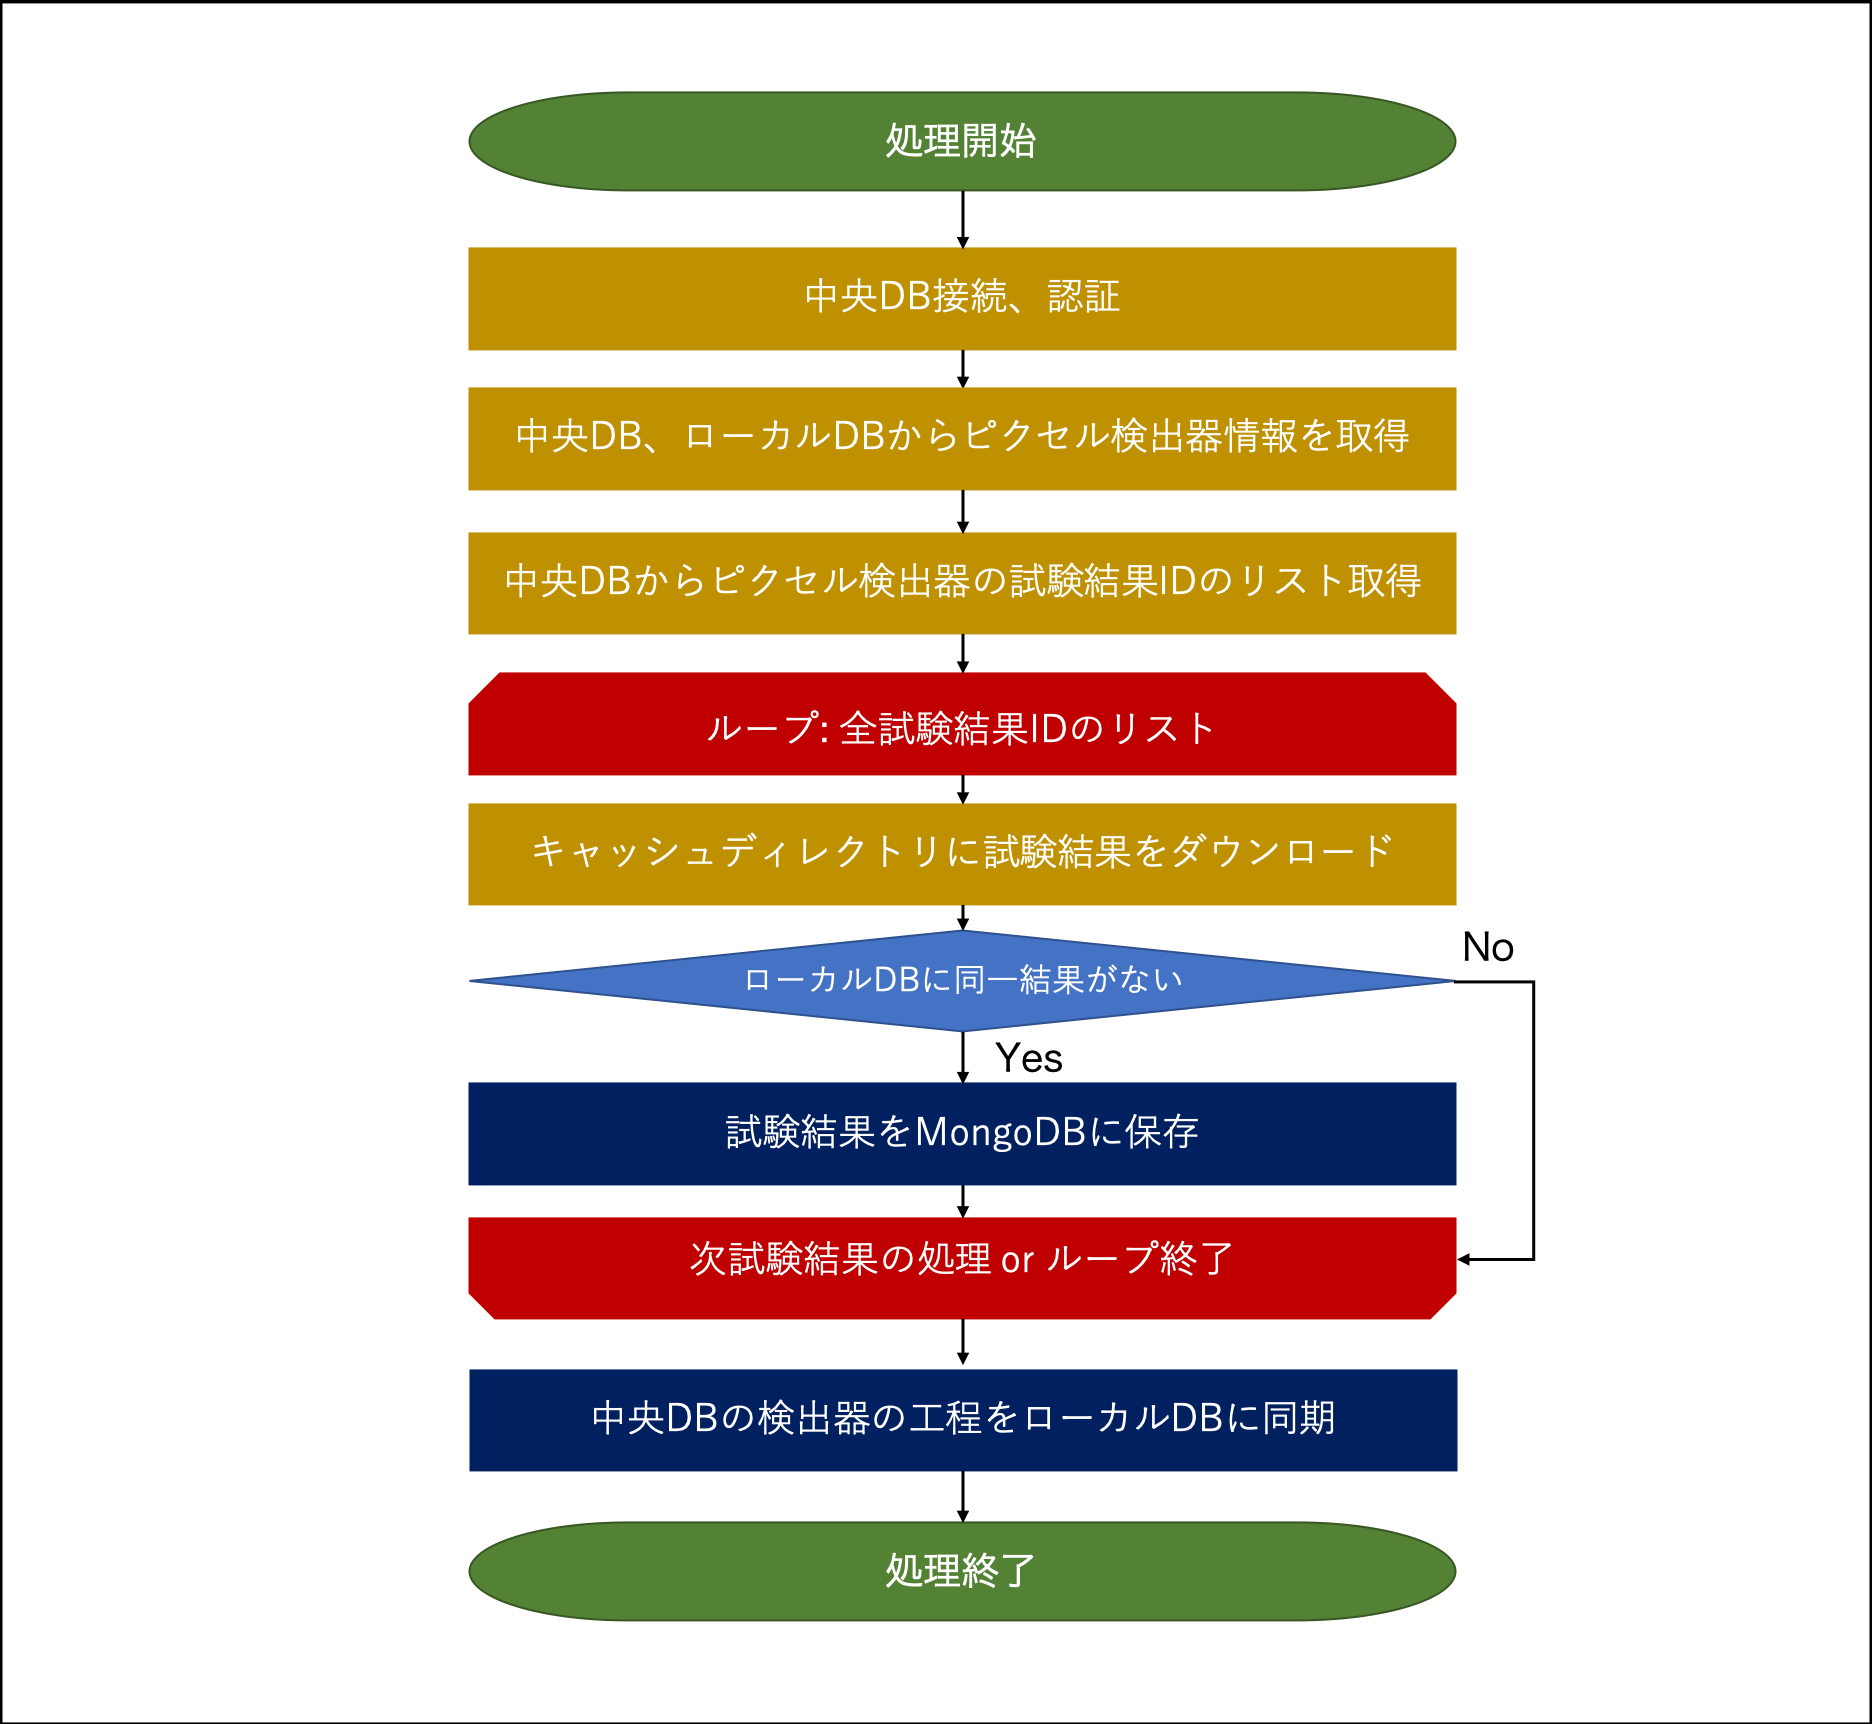
\includegraphics[height=10cm,keepaspectratio]{downloadflow.png}
  \caption[品質試験結果ダウンロード処理の流れ]{品質試験結果ダウンロード処理の流れ。}
  \label{fig:downloadresults}
\end{figure}



%------------------------------------------------------------------------------------------------------------------------
\section{本章のまとめ}
\label{sec:summary7}
%------------------------------------------------------------------------------------------------------------------------

本章では、本研究における開発項目である品質試験結果の表示機能、品質試験結果の管理機能、および中央データベースとローカルデータベースの同期機能についての開発の詳細について述べた。これらの機能をローカルデータベースに実装することにより、ピクセルモジュールの次世代器量産における品質試験結果管理に必要な機能の基本的な部分が全て揃った。

品質試験結果の表示機能について、読み出し試験以外の試験項目についての結果表示機能の開発を行った。読み出し試験結果以外の項目については、品質試験結果登録用GUIを用いてローカルデータベースに登録するため、その開発者と協力しMongoDBのドキュメントの構造の構築をし、ウェブブラウザを用いた結果の表示機能の開発を行った。これにより、ピクセルモジュールの全ての試験項目についての結果を、ウェブブラウザを用いて閲覧可能になった。
また、先行研究で開発された読み出し試験におけるピクセル応答評価機能を拡張し、別の読み出し試験結果と比較する機能の開発を行った。これにより各組み立て工程間における読み出し試験結果の比較を行い、不良ピクセルの変化が確認できる。ピクセル応答評価機能は、デジタル回路やアナログ回路の読み出し試験等のFEチップについてのピクセル評価が行うことができるが、バンプ接続についての評価機能が未実装である。そのため、バンプ接続についての評価機能を実装する必要がある。

品質試験結果の管理機能について、先行研究でピクセルモジュールの組み立て工程の管理及び各工程に対応する品質試験を選択する機能が開発された。これらの機能を拡張し、ワイヤー接続工程の後に確認されるピクセルモジュール特性の更新機能の開発を行った。この機能において選択する品質試験結果は、各組み立て工程における本試験結果であり、中央データベースとの同期機能を用いて同期が行われる。

中央データベースとローカルデータベースの同期機能について、ピクセルモジュールの情報や品質試験結果を中央データベースに共有する機能の開発を行った。この機能を開発するために、中央データベースにおいてピクセルモジュールの構成部品構造や品質試験構造を定義する必要があり、ピクセルモジュール開発グループ内で国際的に議論を行いながら、構造の実装を行った。定義した構造を用いて、ピクセルモジュール情報の登録機能や、品質試験結果のアップロード機能およびダウンロード機能の開発を行った。

品質試験結果のアップロード機能についての性能評価を行った。\tref{tab:sokuteikekka}のように読み出し試験結果以外の項目については数秒でアップロード処理を終えるが、読み出し試験は$160$秒程の処理時間が必要であり、この時間の間にネットワークが不安定になるとバグの原因になりうるため改良が必要である。本研究では処理時間の改善案をいくつか考案し、それぞれについての見積もりを行った。その結果、ローカルデータベースからの読み出し試験結果の抽出処理を並列化することにより、処理時間が最大で$50$秒程度削減できるという結論が得られた。





\newpage
